%%%%%%%%%%%%%%%%%%%%%%%%%%%%%%%%%%%%%%%%%%%%%%%%%%%%%%%%%%%%%%%%%%%%%%%%%%%%%%%%
%% Plantilla de memoria en LaTeX para la ETSIT - Universidad Rey Juan Carlos
%%
%% Por Gregorio Robles <grex arroba gsyc.urjc.es>
%%     Grupo de Sistemas y Comunicaciones
%%     Escuela Técnica Superior de Ingenieros de Telecomunicación
%%     Universidad Rey Juan Carlos
%% (muchas ideas tomadas de Internet, colegas del GSyC, antiguos alumnos...
%%  etc. Muchas gracias a todos)
%%
%% La última versión de esta plantilla está siempre disponible en:
%%     https://github.com/gregoriorobles/plantilla-memoria
%%
%% Para obtener PDF, ejecuta en la shell:
%%   make
%% (las imágenes deben ir en PNG o JPG)

%%%%%%%%%%%%%%%%%%%%%%%%%%%%%%%%%%%%%%%%%%%%%%%%%%%%%%%%%%%%%%%%%%%%%%%%%%%%%%%%

\documentclass[a4paper, 12pt]{book}
%\usepackage[T1]{fontenc}

\usepackage[a4paper, left=2.5cm, right=2.5cm, top=3cm, bottom=3cm]{geometry}
\usepackage{times}
\usepackage[utf8]{inputenc}
\usepackage[spanish]{babel} % Comenta esta línea si tu memoria es en inglés
\usepackage{url}
%\usepackage[dvipdfm]{graphicx}
\usepackage{graphicx}
\usepackage{float}  %% H para posicionar figuras
\usepackage[nottoc, notlot, notlof, notindex]{tocbibind} %% Opciones de índice
\usepackage{latexsym}  %% Logo LaTeX
\usepackage{dirtree}
\usepackage{tikz}
\usepackage{listings}


\usetikzlibrary{shapes,arrows}
\tikzstyle{decision} = [diamond, draw, 
    text width=4.5em, text badly centered, node distance=3cm, inner sep=0pt]
\tikzstyle{block} = [rectangle, draw,  
    text width=5em, text centered, rounded corners, minimum height=4em]
\tikzstyle{line} = [draw, -latex']


\title{Memoria del Proyecto}
\author{Nombre del autor}

\renewcommand{\baselinestretch}{1.5}  %% Interlineado

\begin{document}

\renewcommand{\refname}{Bibliografía}  %% Renombrando
\renewcommand{\appendixname}{Apéndice}

\lstset{frame=L,breaklines=true,keepspaces=true,basicstyle=\footnotesize, language=Python,showstringspaces=false} 

%%%%%%%%%%%%%%%%%%%%%%%%%%%%%%%%%%%%%%%%%%%%%%%%%%%%%%%%%%%%%%%%%%%%%%%%%%%%%%%%
% BIBLIOGRAFIA
\nocite{walter:_learningGuide,appinventordoc:_appinventordoc,pythondoc:_pythondoc,djangodoc:_djangodoc, w3doc:_w3doc,sqldoc:_sqldoc,wwwdoc:_wwwdoc,bootdoc:_bootdoc,boottheme:_boottheme}

%%%%%%%%%%%%%%%%%%%%%%%%%%%%%%%%%%%%%%%%%%%%%%%%%%%%%%%%%%%%%%%%%%%%%%%%%%%%%%%%
% PORTADA

\begin{titlepage}
\begin{center}
\begin{tabular}[c]{c c}
%\includegraphics[bb=0 0 194 352, scale=0.25]{logo} &
\includegraphics[scale=0.25]{img/logo_vect.png} &
\begin{tabular}[b]{l}
\Huge
\textsf{UNIVERSIDAD} \\
\Huge
\textsf{REY JUAN CARLOS} \\
\end{tabular}
\\
\end{tabular}

\vspace{3cm}

\Large
INGENIERÍA DE TELECOMUNICACIÓN Y LICENCIATURA EN ADMINISTRACIÓN Y DIRECCIÓN DE EMPRESAS

\vspace{0.4cm}

\large
Curso Académico 2016/2017

\vspace{0.8cm}

Trabajo Fin de Carrera

\vspace{2.5cm}

\LARGE
MY APP ANALYZER \\
Fomentando la programación de móviles entre los jóvenes

\vspace{4cm}

\large
Autor : Alexandra Ortega Martín \\
Tutor : Dr. Gregorio Robles
\end{center}
\end{titlepage}

\newpage
\mbox{}
\thispagestyle{empty} % para que no se numere esta pagina


%%%%%%%%%%%%%%%%%%%%%%%%%%%%%%%%%%%%%%%%%%%%%%%%%%%%%%%%%%%%%%%%%%%%%%%%%%%%%%%%
%%%% Para firmar
\clearpage
\pagenumbering{gobble}
\chapter*{}

\vspace{-4cm}
\begin{center}
\LARGE
\textbf{Proyecto Fin de Carrera}

\vspace{1cm}
\large
My App Analyzer: Fomentando la programación de móviles entre los jóvenes

\vspace{1cm}
\large
\textbf{Autor :} Alexandra Ortega Martín \\
\textbf{Tutor :} Dr. Gregorio Robles Martínez

\end{center}

\vspace{1cm}
La defensa del presente Proyecto Fin de Carrera se realizó el día \qquad$\;\,$ de \qquad\qquad\qquad\qquad \newline de 2017, siendo calificada por el siguiente tribunal:


\vspace{0.5cm}
\textbf{Presidente:}

\vspace{1.2cm}
\textbf{Secretario:}

\vspace{1.2cm}
\textbf{Vocal:}


\vspace{1.2cm}
y habiendo obtenido la siguiente calificación:

\vspace{1cm}
\textbf{Calificación:}


\vspace{1cm}
\begin{flushright}
Fuenlabrada, a \qquad$\;\,$ de \qquad\qquad\qquad\qquad de 2017
\end{flushright}

%%%%%%%%%%%%%%%%%%%%%%%%%%%%%%%%%%%%%%%%%%%%%%%%%%%%%%%%%%%%%%%%%%%%%%%%%%%%%%%%
%%%% Dedicatoria

\chapter*{}
\pagenumbering{Roman} % para comenzar la numeracion de paginas en numeros romanos
\begin{flushright}
\textit{Dedicado a \\
mi familia \\
gracias por estar siempre ahí}
\end{flushright}

%%%%%%%%%%%%%%%%%%%%%%%%%%%%%%%%%%%%%%%%%%%%%%%%%%%%%%%%%%%%%%%%%%%%%%%%%%%%%%%%
%%%% Agradecimientos

\chapter*{Agradecimientos}
%\addcontentsline{toc}{chapter}{Agradecimientos} % si queremos que aparezca en el índice
\markboth{AGRADECIMIENTOS}{AGRADECIMIENTOS} % encabezado 

Siempre he visto lejano este momento y aunque parecía que nunca iba a llegar, aquí estoy, a punto de poner punto final a mi primer gran paso. Reconozco que tomé la decisión de estudiar la doble licenciatura de forma un poco precipitada, me gustaban demasiadas carreras y no tenía muy claro por qué rama decantarme. Así que cuando vi la posibilidad de unir una ingeniería en la que formarme en varias especialidades con una licenciatura donde me enseñarían cómo funciona la estructura financiera en la que vivimos, supe que era para mí. Por qué no, soy una persona a la que le gustan los retos y el cambio. A día de hoy puedo decir que fue la mejor decisión que he tomado, no sólo porque he cumplido mi objetivo de saber un poquito más de todo, sino porque el perfil multidisciplinar que he desarrollado me ha ayudado muchísimo en mi trayectoria profesional.

Pero no ha sido fácil, ha sido un camino duro del que hubiera salido de no ser por el apoyo de mi familia, son ellos los que han conseguido que hoy pueda estar escribiendo estas líneas. Gracias papá y mamá por esforzaros y ayudarme a estudiar en la universidad, sin vosotros no lo hubiera conseguido. Gracias por empujarme en los momentos de flaqueza, aunque fuera a regañadientes por mi parte. A mi hermano, que con los años hemos descubierto otro punto más en común y siempre me ha animado a seguir mi `vena tecnológica'. Y a mi pareja, quien ha estado conmigo desde el principio, siendo un pilar fundamental en todos estos años y es quien ha sufrido el sprint final. Todas esas noches delante de los apuntes, programando a altas horas de la madrugada o intentando descifrar los problemas de clase han merecido la pena. Ya llegó el final y con él, un nuevo comienzo.

Por último quería agradecer a mi tutor Gregorio Robles la oportunidad de realizar el proyecto con él. Durante la carrera he tenido multitud de profesores, pero al final sólo te acuerdas del nombre de unos pocos, los que realmente han conseguido que su asignatura no sea sólo una más y que realmente te apetezca seguir aprendiendo. Gracias por tu cercanía y paciencia.    

%%%%%%%%%%%%%%%%%%%%%%%%%%%%%%%%%%%%%%%%%%%%%%%%%%%%%%%%%%%%%%%%%%%%%%%%%%%%%%%%
%%%% Resumen

\chapter*{Resumen}
%\addcontentsline{toc}{chapter}{Resumen} % si queremos que aparezca en el índice
\markboth{RESUMEN}{RESUMEN} % encabezado

\textbf{My App Inventor} es una aplicación web que permite analizar y clasificar proyectos realizados en App Inventor, una plataforma de desarrollo de aplicaciones móviles para el sistema operativo Android.

A través de un diseño atractivo y una navegación sencilla, el \textbf{objetivo} de este proyecto es orientar a los futuros programadores y mejorar su pensamiento computacional. Analizaremos tres aspectos clave de las aplicaciones creadas con App Inventor: componentes utilizados, técnicas de programación aplicadas y usabilidad, y mostraremos los resultados al usuario de forma que no sólo obtenga su nivel, sino que también conozca cómo mejorarlo. 
 
Las múltiples \textbf{tecnologías} utilizadas para llevar a cabo este proyecto está orientadas al desarrollo web. Desde el lado del servidor, como base de la aplicación se han utilizado el lenguaje Python 2.7 y su framework Django 1.9., junto con la base de datos SQLite. Centrándonos en la capa \textit{Front end} donde se encuentra el cliente, además de HTML y CSS se ha añadido dinamismo a la web con Bootstrap, JavaScript y AJAX, adaptándola a las nuevas tendencias de maquetación.  


%%%%%%%%%%%%%%%%%%%%%%%%%%%%%%%%%%%%%%%%%%%%%%%%%%%%%%%%%%%%%%%%%%%%%%%%%%%%%%%%
%%%% Resumen en inglés

\chapter*{Summary}
%\addcontentsline{toc}{chapter}{Summary} % si queremos que aparezca en el índice
\markboth{SUMMARY}{SUMMARY} % encabezado

\textbf{My App Inventor} is a web application that analyze and classify projects done in App Inventor, a development platform focused in mobile applications based on Android. 

Through an attractive design and easy navigation, the \textbf{objetive} of this project is to guide future developers and improve its computational thinking. We analize three key points of the apps created with App Inventor: componentes included, applied programming techniques and schedule, displaying the results to the users so that they don't only know their level but also offer tips to improve it. 

The multiple \textbf{technologies} used in this project are oriented towards web development. At the server side, Python 2.7 and its framework Django 1.9 have been used together with data base SQLite. In the Front end, where the client is located, in addition to HTML and CSS, Bootstrap, JavaScript and AJAX have been included to dinamize the templates and adapt them to the new layout trends.

%%%%%%%%%%%%%%%%%%%%%%%%%%%%%%%%%%%%%%%%%%%%%%%%%%%%%%%%%%%%%%%%%%%%%%%%%%%%%%%%
%%%%%%%%%%%%%%%%%%%%%%%%%%%%%%%%%%%%%%%%%%%%%%%%%%%%%%%%%%%%%%%%%%%%%%%%%%%%%%%%
% ÍNDICES %
%%%%%%%%%%%%%%%%%%%%%%%%%%%%%%%%%%%%%%%%%%%%%%%%%%%%%%%%%%%%%%%%%%%%%%%%%%%%%%%%

% Las buenas noticias es que los índices se generan automáticamente.
% Lo único que tienes que hacer es elegir cuáles quieren que se generen,
% y comentar/descomentar esa instrucción de LaTeX.

%%%% Índice de contenidos
\tableofcontents 
%%%% Índice de figuras
\cleardoublepage
%\addcontentsline{toc}{chapter}{Lista de figuras} % para que aparezca en el indice de contenidos
\listoffigures % indice de figuras
%%%% Índice de tablas
%\cleardoublepage
%\addcontentsline{toc}{chapter}{Lista de tablas} % para que aparezca en el indice de contenidos
%\listoftables % indice de tablas


%%%%%%%%%%%%%%%%%%%%%%%%%%%%%%%%%%%%%%%%%%%%%%%%%%%%%%%%%%%%%%%%%%%%%%%%%%%%%%%%
%%%%%%%%%%%%%%%%%%%%%%%%%%%%%%%%%%%%%%%%%%%%%%%%%%%%%%%%%%%%%%%%%%%%%%%%%%%%%%%%
% INTRODUCCIÓN %
%%%%%%%%%%%%%%%%%%%%%%%%%%%%%%%%%%%%%%%%%%%%%%%%%%%%%%%%%%%%%%%%%%%%%%%%%%%%%%%%

\cleardoublepage
\chapter{Introducción}
\label{sec:intro} % etiqueta para poder referenciar luego en el texto con ~\ref{sec:intro}
\pagenumbering{arabic} % para empezar la numeración de página con números

En una época donde las nuevas tecnologías están totalmente integradas en nuestro día a día y en la que los niños cada vez aprenden antes a usar ordenadores y móviles, es importante desarrollar en los más jóvenes aptitudes lógicas que les conviertan de simples consumidores a creadores. 
Como futuros informáticos, médicos, profesores o dibujantes, el pensamiento computacional les ayudará a pensar de una forma organizada, metódica y secuencial, capacidades que les serán de ayuda sea cual sea su profesión. Pero ¿cómo podemos enseñarles informática cuando son tan pequeños? Las metodologías clásicas de aprendizaje en las que la principal barrera de entrada es un lenguaje complicado y abstracto han dado paso a nuevas formas de enseñar a programar donde aplicaciones sencillas y con un diseño atractivo permiten a los jóvenes `aprender jugando'.

\section{Marco General}
\label{subsec:marcogral}
Ya en la década de los 60 se detectó la necesidad de acercar la tecnología a la sociedad con Logo\footnote{\url{http://el.media.mit.edu/logo-foundation/what_is_logo/history.html}}, un lenguaje simple donde por medio de instrucciones básicas se guiaba a una tortuga para crear formas geométricas en la pantalla.
Logo fue el precursor de los nuevos lenguajes y aplicaciones como Blockly\footnote{\url{https://developers.google.com/blockly/}} y su metodología de interconexión de bloques, Scratch\footnote{\url{https://scratch.mit.edu/}}, App Inventor o Alice\footnote{\url{http://www.alice.org/index.php}}, donde podemos crear animaciones en 3D.
\begin{figure}[H]
  \centering
  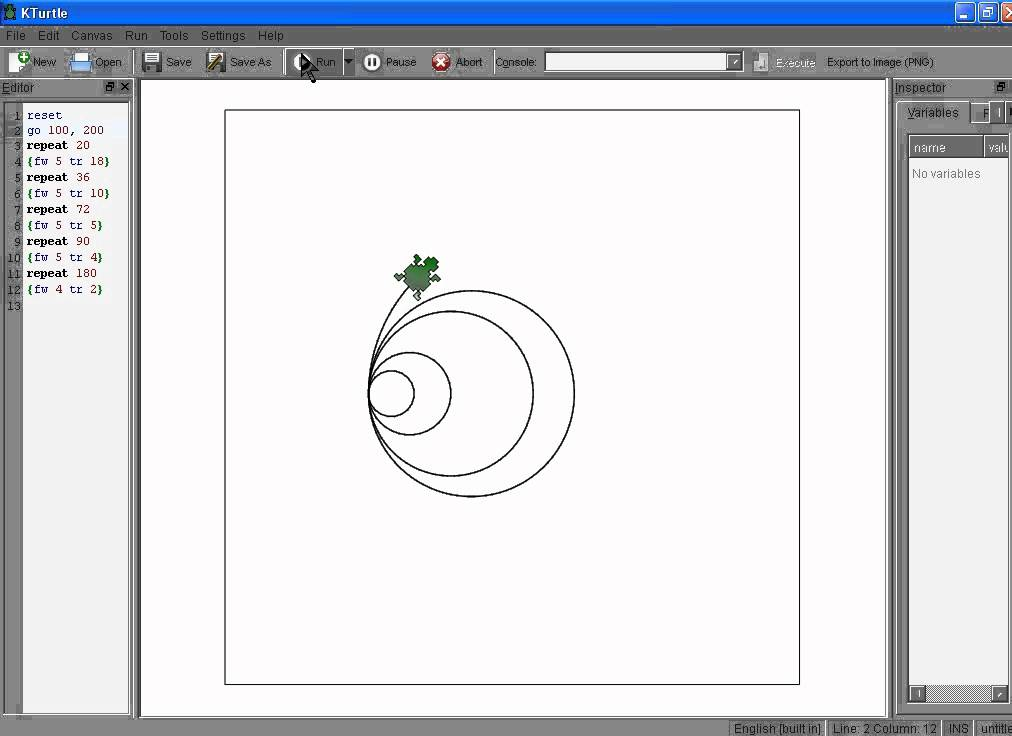
\includegraphics[width=0.60\linewidth, keepaspectratio]{img/logoProgramm}
  \caption{Programación con Logo}
  \label{fig:logoProgramm}
\end{figure} 

Siguiendo la idea de mis compañeros de carrera y su proyecto Dr. Scratch\footnote{\url{http://www.drscratch.org/}}, mi tutor Gregorio Robles me propuso crear una línea paralela de trabajo donde poder continuar con la labor educativa de esta aplicación pero centrándonos en otro modelo de programación. Tras analizar las alternativas, elegimos App Inventor, que mantiene la metodología de programación por bloques de Scratch o Blockly enfocándola a un público de mayor edad. 
\begin{figure}[H]
  \centering
  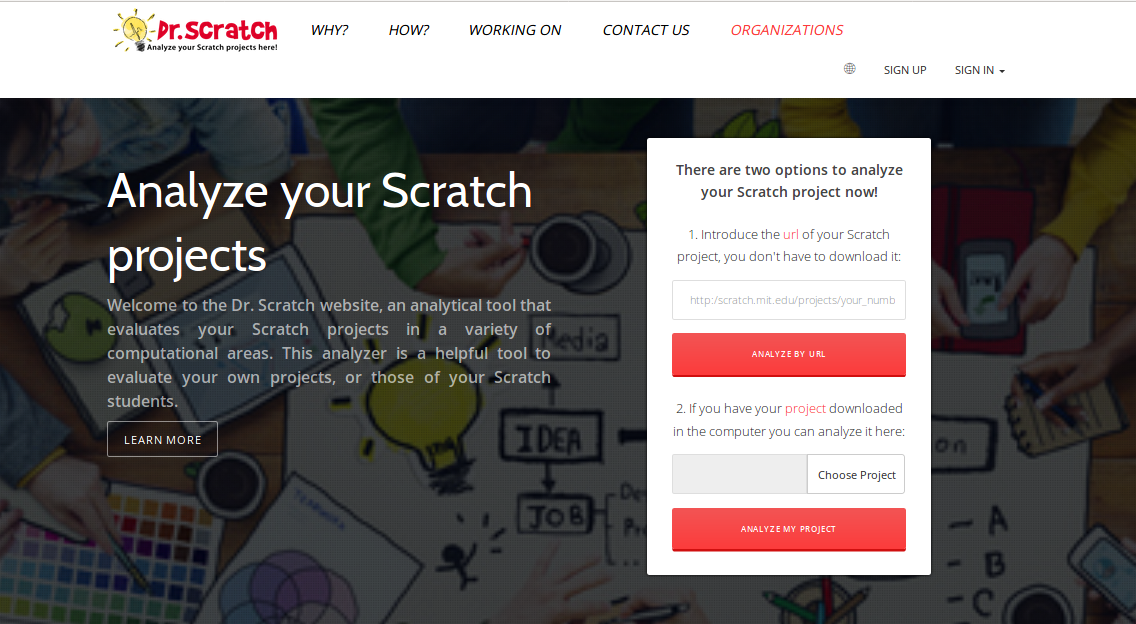
\includegraphics[width=0.70\linewidth, keepaspectratio]{img/DrScratch}
  \caption{Dr. Scratch}
  \label{fig:DrScratch}
\end{figure}
Dr. Scratch es una aplicación web que analiza programas creados en Scratch. Tomando como base la librería Hairball\footnote{\url{https://github.com/ucsb-cs-education/hairball}}, muestra información sobre aspectos del pensamiento computacional tales como pensamiento lógico, control de flujo, abstracción, paralelismo, sincronización\ldots Ofreciendo una puntuación al usuario que le servirá de guía para conocer el nivel de su programa. Los puntos clave del análisis vienen determinados por las posibilidades que ofrece Scratch respecto a bloques y configuración, que varían respecto a los que nos encontramos en App Inventor. 
Otra diferencia notable entre Scratch y App Inventor la encontramos en la salida que proporcionan. Mientras que el primero está enfocado a aplicaciones web, el segundo se centra en las aplicaciones para móviles Android. Además, como hemos comentado anteriormente, App Inventor está dirigido a un público joven, ofreciéndole la posibilidad de utilizar el hardware de sus \emph{smartphones}, como la cámara o el \emph{Bluetooth}, e incluso interactuar con robots Lego Mindstorms.

\section{Estructura de la memoria}
\label{sec:estructura}

A continuación veremos la estructura de esta memoria y sus capítulos principales:

\begin{itemize}
  \item Introducción: presentación del trabajo y del contexto social en el que se desarrolla, además de la motivación para afrontarlo.
  
  \item Objetivos: desarrollo de qué es lo que buscamos con nuestra aplicación y los pasos seguidos para obtener el resultado final. 
  
  \item Estado del arte: breve introducción a las principales tecnologías utilizadas. 
  
  \item Diseño e implementación: arquitectura de My App Inventor, funcionalidades y cómo se han utilizado las diferentes tecnologías. Incluye un manual de usuario. 

  \item Resultados: análisis del resultado final del proyecto. 

  \item Conclusiones: reflexión sobre los resultados obtenidos, consecución de objetivos y problemas encontrados.
\end{itemize}



%%%%%%%%%%%%%%%%%%%%%%%%%%%%%%%%%%%%%%%%%%%%%%%%%%%%%%%%%%%%%%%%%%%%%%%%%%%%%%%%
%%%%%%%%%%%%%%%%%%%%%%%%%%%%%%%%%%%%%%%%%%%%%%%%%%%%%%%%%%%%%%%%%%%%%%%%%%%%%%%%
% OBJETIVOS %
%%%%%%%%%%%%%%%%%%%%%%%%%%%%%%%%%%%%%%%%%%%%%%%%%%%%%%%%%%%%%%%%%%%%%%%%%%%%%%%%

\cleardoublepage
\chapter{Objetivos}
\label{chap:objetivos}

\section{Objetivo general}
\label{sec:objetivo-general} El objetivo general de este proyecto es crear una plataforma donde los nuevos programadores puedan evaluar su código de forma que no sólo puedan conocer sus puntos fuertes y débiles sino que además puedan obtener nuevos retos para mejorar sus habilidades computacionales. 

Niños y jóvenes con interés por la programación conforman el público objetivo al que va destinada la aplicación. Por ello se han adaptado el diseño, funcionalidad y lenguaje para que resulten la experiencia de usuario sea lo más atractiva y lúdica posible. 

En el sistema de clasificación hemos huido de las puntuaciones numéricas, convirtiéndolas en tres niveles representados por los colores del semáforo: alto (verde), medio (amarillo) y bajo (rojo). De esta manera convertimos la experiencia en un juego, enmarcándola en un contexto más positivo para el usuario y alejándonos de las puntuaciones numéricas utilizadas de los exámenes. 

Toda la aplicación se relaciona con el usuario a través de un lenguaje coloquial, sencillo y en inglés. Se eligió este idioma porque es importante familiarizar a los niños con el mismo y reforzar sus conocimientos a través del juego.

\section{Objetivos específicos}
\label{sec:objetivos-especificos}
\begin{itemize}
  \item Analizar las posibilidades de personalización y bloques computacionales que ofrece App Inventor como herramienta para crear programas.

  \item Definir las habilidades y capacidades del usuario a analizar. De los múltiples enfoques considerados y de cara a una simplificación de la información final se optó por crear tres grandes bloques de análisis: componentes, programación y usabilidad.

  \item Crear una aplicación Django donde se recoja la lógica anterior y poder ofrecer al usuario la información de manera clara y resumida. El usuario podrá además tener un registro de los proyectos guardados con anterioridad para poder revisar su clasificación. 
  
  \item Unir las tecnologías Django, Bootstrap y AJAX para mejorar la capa de \textit{Front End} y hacer la experiencia de usuario mucho más dinámica.   
\end{itemize}


\section{Planificación temporal}
\label{sec:planificacion-temporal}
La planificación temporal del proyecto ha sido definida en función de los objetivos específicos marcados siguiendo un orden que permitiera avanzar en todos los aspectos de la aplicación:
\begin{itemize}
  \item \textbf{Fase I}: búsqueda de documentación sobre App Inventor y creación de una cuenta en su web\footnote{\url{http://appinventor.mit.edu/explore/}} donde poder analizar los bloques disponibles para el usuario, el contenido del archivo comprimido (\textit{.aia}) en que se guardan los programas y cómo se representa la información dentro del mismo. Comencé esta fase en agosto de 2016.

  \item \textbf{Fase II}: entre septiembre de 2016 y febrero de 2017 realicé las siguientes tareas:
	\begin{itemize}
		\item Creación de una aplicación Django con una web simple donde subir el fichero con el proyecto, descomprimirlo y guardar su información en base de datos.
		\item Añadir la posibilidad de tener una cuenta de usuario en la aplicación donde se almacenen los diferentes proyectos subidos de cara a futuras consultas. 
	\end{itemize}
  \item \textbf{Fase III}: definición de los puntos a analizar en cada proyecto subido e implementar la lógica de evaluación y clasificación. Esta parte del proyecto fue desarrollada entre febrero y marzo de 2017.
  
  
  \item \textbf{Fase IV}: incorporar a la web las tecnologías Bootstrap y AJAX para añadir dinamismo y mejorar su aspecto.  La última fase ocupó los meses de abril y mayo, donde comencé a a escribir la memoria. 
\end{itemize}


%%%%%%%%%%%%%%%%%%%%%%%%%%%%%%%%%%%%%%%%%%%%%%%%%%%%%%%%%%%%%%%%%%%%%%%%%%%%%%%%
%%%%%%%%%%%%%%%%%%%%%%%%%%%%%%%%%%%%%%%%%%%%%%%%%%%%%%%%%%%%%%%%%%%%%%%%%%%%%%%%
% ESTADO DEL ARTE %
%%%%%%%%%%%%%%%%%%%%%%%%%%%%%%%%%%%%%%%%%%%%%%%%%%%%%%%%%%%%%%%%%%%%%%%%%%%%%%%%

\cleardoublepage
\chapter{Estado del arte}
En este capítulo se explicarán brevemente las principales tecnologías utilizadas en el proyecto.
\section{App Inventor} 
\label{sec:seccion1}
MIT App Inventor es un entorno de desarrollo web para la creación de aplicaciones móviles basadas en el sistema Android. Su principal objetivo es democratizar la programación y acercarla al público más joven transformándolo de consumidor de tecnología, a creador de la misma.
\begin{center}
        \textit{`Anyone Can Build Apps That Impact the World'}
\end{center}
\begin{figure}[H]
  \centering
  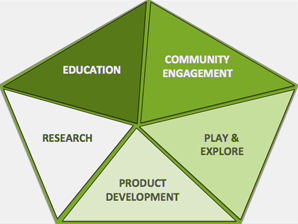
\includegraphics[width=0.40\linewidth, keepaspectratio]{img/usesview}
  \caption{Web App Inventor}
  \label{fig:appinventorgallery}
\end{figure}
Gracias a su entorno gráfico sencillo e intuitivo, permite la construcción gratuita de programas reduciendo la curva de aprendizaje y eliminando barreras de entrada ya que para utilizarlo sólo es necesario un ordenador con internet y un móvil con sistema operativo Android. Pero además de las ventajas desde el punto de vista tecnológico también hay que añadir el componente social. En su web nos permiten no sólo subir el código sino que además se pueden ver y descargar gratuitamente los programas de otros usuarios para usarlos o modificarlos. Desde su creación en 2015 es utilizado en colegios para mejorar la visión lógica de los estudiantes y crear comunidades educativas que conectan a jóvenes de cualquier parte del mundo. 
\begin{figure}[H]
  \centering
  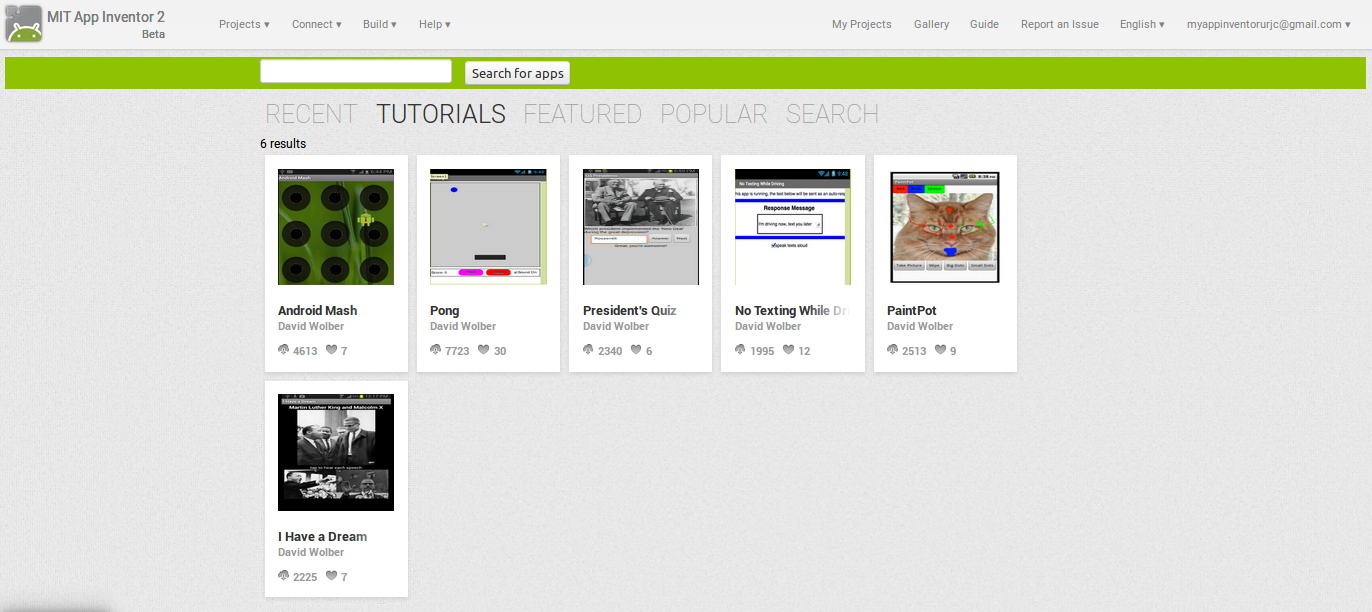
\includegraphics[width=0.90\linewidth, keepaspectratio]{img/appinventorgallery}
  \caption{Web App Inventor}
  \label{fig:appinventorgallery}
\end{figure} 
Para poder utilizarlo hay que tener una cuenta de Google y entrar en su web\footnote{\url{http://appinventor.mit.edu/explore/}}. Tras iniciar sesión y seleccionar la aplicación, disponemos de dos herramientas: Designer y Blocks. Ambas funcionan con de la funcionalidad \textit{drag \& drop}, una vez decidido qué componente o bloque utilizar, lo arrastraremos hasta la previsualización de pantalla (\textit{Viewer}) para situarlo en una zona determinada o conectarlo con otros elementos.
\subsection{App Inventor Designer} 
En este apartado se construye la interfaz de usuario del programa, añadiendo y personalizando los componentes. 
\begin{figure}[H]
  \centering
  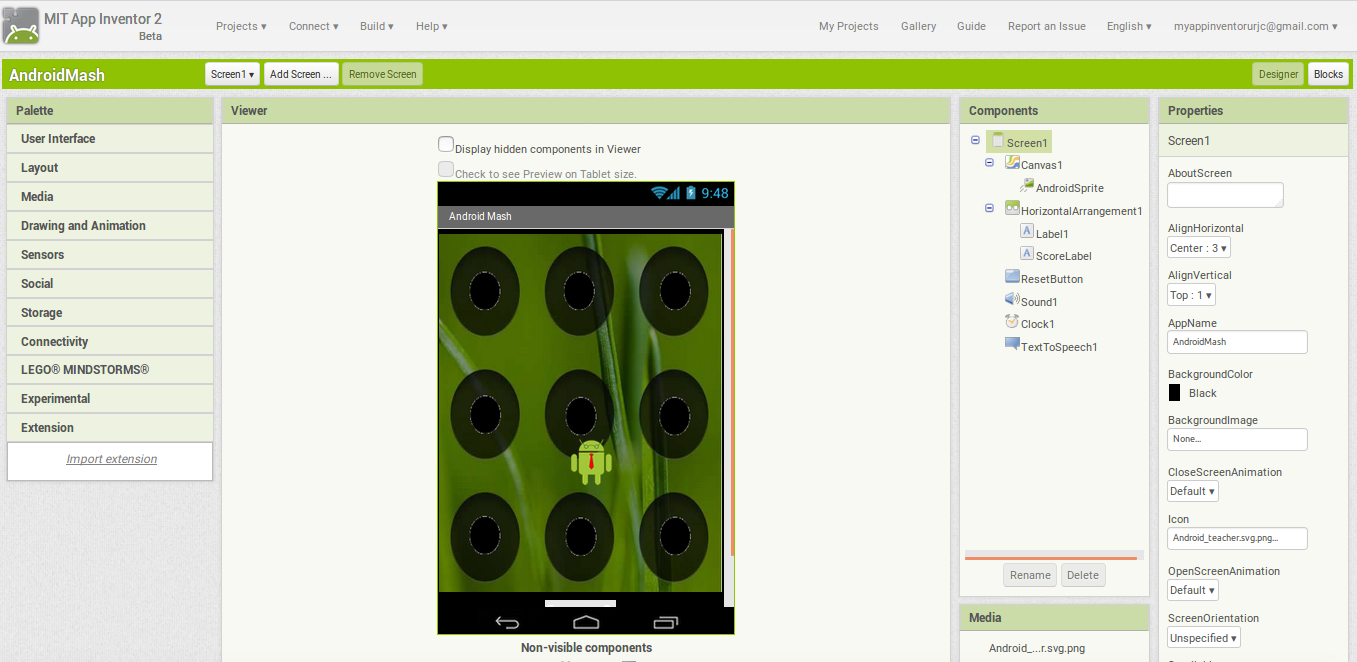
\includegraphics[width=\linewidth, keepaspectratio]{img/appDesigner}
  \caption{Web App Inventor}
  \label{fig:appinventorgallery}
\end{figure}
Incluye una amplia librería que nos permite escoger entre componentes de distinta complejidad y que serán objeto de análisis en nuestra aplicación como veremos en el siguiente capítulo:
\begin{itemize}		
\item \textit{User Interface}: botones, imágenes, casillas y todo tipo de elementos que forman parte de la interfaz de usuario y forman la estructura básica del programa.
\item \textit{Layout}: crea secciones horizontales o verticales en la pantalla. 
\item \textit{Media}: cámara de fotos o vídeo, reproductor de audio, grabadora\ldots 
\item \textit{Drawing and animation}: paneles de dibujo o delimitador de zonas para interactuar con el usuario a través de la pantalla táctil.
\item \textit{Sensors}:	reloj, geolocalizador, podómetro, sensor de proximidad\ldots 
\item \textit{Social}: permite acceder a la lista de contactos, compartir ficheros o texto e incluso conectarse a Twitter. 
\item \textit{Storage}:	con gestores de ficheros y bases de datos.
\item \textit{Connectivity}: creación de servidor/cliente de Bluetooth y posibilidad de realizar peticiones HTTP.	
\item \textit{Lego Mindstorms}\footnote{\url{https://www.lego.com/en-gb/mindstorms/}}: interfaz de alto nivel para controlar los componentes de los robots Lego.
\item \textit{Experimental}: como alternativa al almacenamiento de datos incluido en \textit{Storage}, se puede incluir Firebase\footnote{\url{https://firebase.google.com/}}, una base de datos creada por Google optimizada para dispositivos móviles.
\item \textit{Extension}: importador de extensiones de terceros. 
\end{itemize}
\subsection{App Inventor Blocks} 
Todo en App Inventor está causado por un evento: el click en un botón, la finalización de un reloj, el inicio de una conexión\ldots Tras crear la máscara de la aplicación con los componentes, la dotaremos de lógica en la vista Blocks. 
\begin{figure}[H]
  \centering
  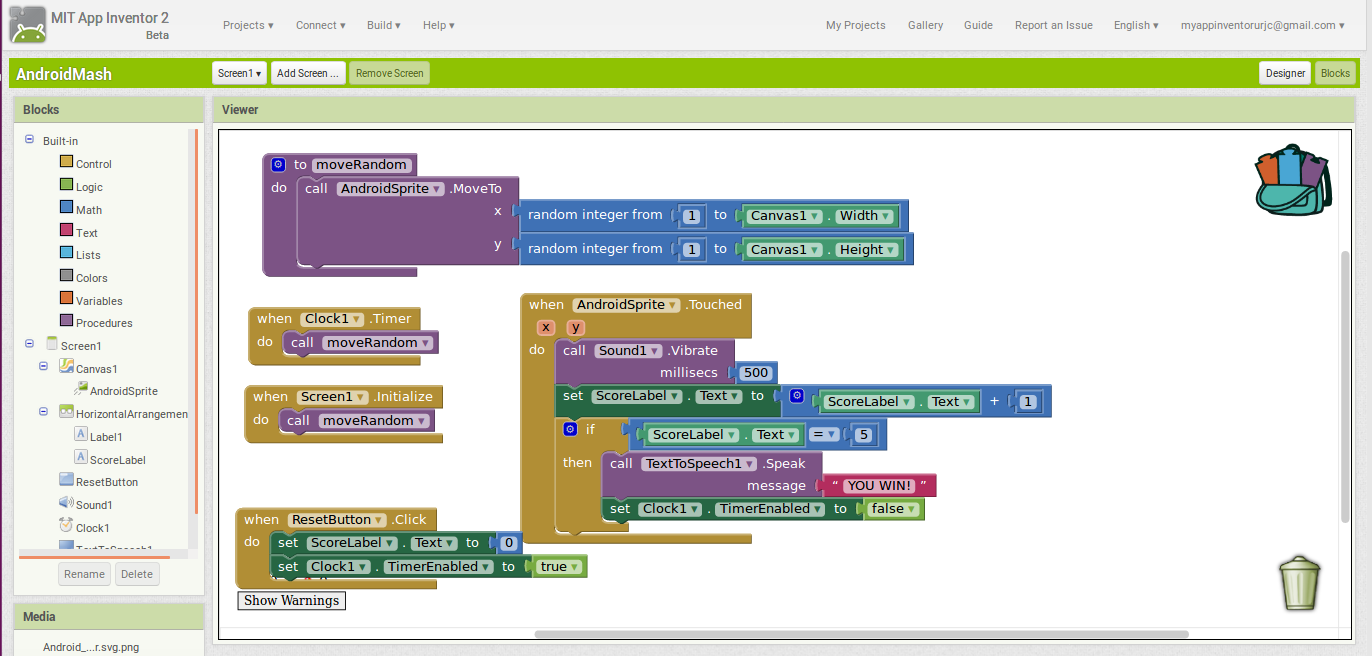
\includegraphics[width=\linewidth, keepaspectratio]{img/appBlock}
  \caption{Web App Inventor}
  \label{fig:appinventorgallery}
\end{figure}
Por pantalla podremos insertar: 
\begin{itemize}	
	\item \textit{Built-in}: bloques lógicos predefinidos que podemos combinar entre sí:
		\begin{itemize}	
		\item \textit{Control}: condicionales y bucles.
		\item \textit{Logic}: comparadores, booleanos (\textit{Strue/false}) y puertas lógicas (\textit{and/or})	
		\item \textit{Math}: operaciones matemáticas algebraicas y trigonométricas.	
		\item \textit{Text}: funciones para variables tipo texto: contiene, longitud, concatenación\ldots	
		\item \textit{Lists}: creación, consulta y modificación de listas de variables. 	
		\item \textit{Colors}: selector de color.
		\item \textit{Variables}: creación, inicialización y modificación de variables locales y globales.
		\item \textit{Procedures}: definición de procedimientos
		\end{itemize}
	\item \textit{Screen}: gestión de eventos sobre los componentes añadidos en cada pantalla. 
	\item \textit{Any Component}: gestión de eventos globales por componente. Por ejemplo, podemos definir una acción a ejecutar cuando se pulse un botón en cualquiera de las pantallas que componen el programa.  

\end{itemize}

\section{Python} 
\label{sec:seccion2}
Python es un potente lenguaje de programación de alto nivel entre cuyas características principales destaca una: la sencillez. Gracias a su facilidad de uso y de lectura, cualquier programador puede entender su sintaxis y adaptarla a sus necesidades. Además es de código abierto y multiplataforma, es decir, puede redistribuirse gratuitamente en cualquier sistema operativo: Linux, Unix, Windows o MAC OS.
\begin{figure}[H]
  \centering
  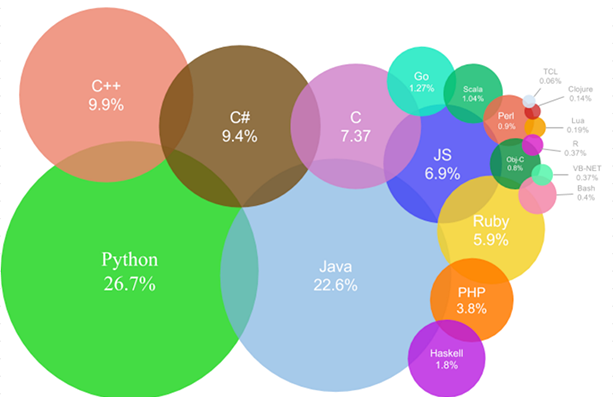
\includegraphics[width=0.70\linewidth, keepaspectratio]{img/codeval2016}
  \caption{Lenguajes más importantes en 2016. Fuente: www.codeeval.com}
  \label{fig:codeval2016}
\end{figure}
Algunas características a destacar:
\begin{itemize}
	\item Sintaxis sencilla: como hemos comentado, se busca una escritura simple, reduciendo caracteres redundantes y favoreciendo su interpretación rápida. Como ejemplo de esto, la definición de los bloques por el nivel del sangrado (eliminando llaves o delimitadores de fin de instrucción) o la sustitución de los caracteres lógicos \&\&, \(\vert \vert\) y ! por palabras como \textit{and, or} y \textit{not}.   	
	\item Incluye multitud de librerías optimizadas para reducir el código y el tiempo de ejecución.
	\item Dinámicamente tipado: no es necesario definir los tipos de datos previamente sino que podemos ir añadiendo variables y automáticamente Python les asignará un tipo en función de su contenido. 
	\item Fuertemente tipado: no convierte automáticamente unos tipos de datos en otros.
	\item Incluye un modo interactivo donde poder ver el resultado de las instrucciones inmediatamente sin necesidad de compilar previamente el programa.
	\item Soporta programación orientada a objetos.
	\item Puede extenderse añadiendo módulos implementados en otros lenguajes como C o C++. 
\end{itemize}

\section{Django} 
\label{sec:seccion3}
Django es un framework de alto nivel escrito en Python para construir aplicaciones web de forma gratuita, sencilla y rápida. Incluye todas las librerías necesarias que pueden utilizarse en el desarrollo web, de manera que el programador sólo tiene que preocuparse en diseñar su aplicación sin necesidad de `reinventar la rueda'.

Principales características:
\begin{itemize}
	\item Rápido: las funciones están optimizadas para que su ejecución sea lo más rápida posible.
	\item Seguro: ayuda a los desarrolladores a evitar los errores más comunes en seguridad.  
	\item Escalable: es flexible y fácilmente escalable, adaptándose a las necesidades de la aplicación. 
	\item Código abierto: el uso de funciones predefinidas no excluye que el programador tenga acceso a su contenido para reutilizar o modificarlas. Todo el código es accesible para los usuarios. 
	\item Versátil: gracias a Django podemos crear todo tipo de aplicaciones como servidores de contenidos (\url{www.openstack.org}) o redes sociales(\url{www.instagram.com}).
\end{itemize}
\section{SQLite} 
\label{sec:seccion4}
SQLite es un sistema de gestión de bases de datos basado en el estándar SQL. Sus principales características son:
\begin{itemize}
	\item Transacciones atómicas, consistencia, aislamiento, y durabilidad ante fallos de sistema. 
	\item No necesita configuración previa para poder utilizarlo.
	\item Multiplataforma: Android, BSD, iOS, Linux, Mac, Solaris, VxWorks y Windows
	\item No es una parte independiente del programa con el que se comunica sino que se integra con él, reduciendo la latencia de acceso. La base de datos se guarda como un fichero estándar dentro del sistema. 
	\item De dominio público. 
\end{itemize}
\section{HTTP} 
\label{sec:seccion5}
HTTP son las siglas de Hypertext Transfer Protocol, un protocolo de comunicación web a nivel aplicación. Se utiliza en aplicaciones distribuidas y define los mensajes a intercambiar entre cliente y servidor dentro del protocolo pregunta/respuesta.  
\begin{itemize}
	\item No mantiene estado: no guarda información de conexiones anteriores. En caso de necesitar hacerlo se utilizan cookies, ficheros de información almacenados en el cliente por el servidor. 
	\item Es colaborativo. 
	\item Los mensajes enviados están escritos en texto plano y siguen la estructura:
	\begin{itemize}
		\item Método de petición + URL del recurso + versión HTTP del cliente. Concretamente en nuestra aplicación usaremos los métodos GET para petición simple de recursos (solicitar una página web) y POST para envío de datos de cara a su procesamiento (envío de datos de formulario). 
		\item Cabecera con metadatos: idioma, tipo de servidor, fecha, cookie\ldots
		\item Cuerpo con datos a intercambiar.
	\end{itemize}	
\end{itemize}
\section{HTML5} 
\label{sec:seccion6}
\textit{HyperText Markup Language} o HTML es el lenguaje estándar de la World Wide Web (WWW) en el que se define el formato para elaborar las páginas web. Está basado en ficheros de texto plano donde la interpretación del código recaerá sobre el navegador del cliente, que será el encargado de solicitar los recursos especificados y mostrar el contenido correctamente. 

Los ficheros HTML utilizan etiquetas y atributos para identificar cada elemento del documento:
\begin{lstlisting}[language=HTML]
<!DOCTYPE HTML> 
<html>
  <head>
    <title>App Inventor Analyzer</title>
  </head>
  <body>
    <p>Cuerpo de la web</p>
  </body>
</html>
\end{lstlisting}
Actualmente se encuentra en la versión 5 cuyas principales novedades permiten mayor dinamismo en las páginas web: etiquetas para 2D y 3D, generación de tablas dinámicas, nuevos tipos de datos en formularios o funcionalidad Drag \& Drop. 
\section{CSS} 
\label{sec:seccion7}
\textit{Cascading Style Sheets} o CSS es un lenguaje de diseño gráfico utilizado para dar estilo a ficheros HTML y XML. A través de la separación entre contenido y formato permiten eliminar líneas redundantes en los documentos, realizar modificaciones globales más fácilmente y adaptar la visualización para diferentes métodos de renderizado. 
Para utilizar CSS se necesita:
 	\begin{itemize}	
		\item Fichero .css: en el se definen las reglas mediante pares selector - bloque de declaración.
		\begin{lstlisting}[language=HTML]
header .intro-text .intro-heading {
  font-family: "Montserrat", "Helvetica Neue", Helvetica, Arial, sans-serif;
  text-transform: uppercase;
  font-weight: 700;
  font-size: 50px;
  margin-bottom: 25px;}
		\end{lstlisting}
		\item Fichero .html: donde se identifican los elementos a formatear con el selector especificado en el fichero .css.
		\begin{lstlisting}[language=HTML]
<div class="intro-text">
	<div class="intro-lead-in">Welcome to MIT App Inventor Analyzer</div>
	<div class="intro-heading">It's Nice To Meet You</div>
	<a href="#services" class="page-scroll btn btn-xl">Tell Me More</a>
</div>
		\end{lstlisting}
	\end{itemize}
\section{JavaScript} 
\label{sec:seccion8}
JavaScript es un lenguaje de programación interpretado utilizado principalmente en el lado del cliente para añadir dinamismo a las páginas web mostradas por el navegador. Al ser interpretado, no necesita ser compilado previamente ya que se interpreta a tiempo real, mejorando la eficiencia de las aplicaciones. 
\section{Bootstrap} 
\label{sec:seccion9}
Bootstrap es un framework de código abierto para el desarrollo de páginas y aplicaciones web creado por desarrolladores de Twitter. Este conjunto de herramientas une las tecnologías HTML, CSS, y Javascript para adaptar dinámicamente el formato de las webs al dispositivo utilizado (ordenador, tableta o móvil).
La estructura básica de Bootstrap sigue el sistema de ficheros de la figura~\ref{fig:dirarchivosBoot}. En ella podemos ver cómo los ficheros CSS y JavaScript base vienen incluidos en su versión normal (*.css) y minimizada (*.min.css). Esta última es una compresión en la que se eliminan caracteres innecesarios en el código como espacios o saltos de línea, y su objetivo es reducir el tiempo de procesado de los ficheros por el navegador. 
\begin{figure}[H]
  \dirtree{%
	.1 bootstrap.
	.2 css.
	.3 bootstrap.css.
	.3 bootstrap.min.css.
	.2 js.
	.3 bootstrap.js.
	.3 bootstrap.min.js.
	.2 img.
	.3 glyphicons-halflings.png.
	.3 glyphicons-halflings-white.png.
	}
  \caption{Directorio de archivos Bootstrap}
  \label{fig:dirarchivosBoot}
\end{figure}
\begin{figure}[H]
	\begin{center}
	    \begin{tabular}{ p{0.50\linewidth} p{0.50\linewidth}  }
	    \hline
	    \textbf{HTML simple} & \textbf{HTML con Bootstrap}  \\ \hline
	    	\begin{lstlisting}[language=HTML]
<!DOCTYPE html>
<html>
<head>
<title>Bootstrap 101 Template</title>
</head>
<body>
<h1>Hello, world!</h1>
<script src="http://code.jquery.com/jquery.js"></script>
</body>
</html>
		\end{lstlisting} & 
	    	\begin{lstlisting}[language=HTML]
<!DOCTYPE html>
<html>
<head>
<title>Bootstrap 101 Template</title>
<!-- Bootstrap -->
<link href="css/bootstrap.min.css" rel="stylesheet" media="screen">
</head>
<body>
<h1>Hello, world!</h1>
<script src="http://code.jquery.com/jquery.js"></script>
<script src="js/bootstrap.min.js"></script>
</body>
</html>
		\end{lstlisting}\\ 
            \end{tabular}
	\end{center}
	\caption{HTML simple VS. con Bootstrap }
	\label{fig:htmlcomparison}
\end{figure}
\section{AJAX} 
\label{sec:seccion10}
\textit{Asynchronous JavaScript And XML} o AJAX es una técnica de desarrollo asíncrona para actualización de páginas web bajo petición sin necesidad de recargarlas completamente, lo que mejora la eficiencia de las aplicaciones. Utilizando AJAX podemos utilizar varias tecnologías: HTML (datos), CSS (estilo), Document Object Model o DOM (actualización dinámica de contenido), HTMLHttpRequest (petición al servidor) y XML (formato de envío de información).

En nuestra aplicación My App Inventor podemos ver un ejemplo de esta tecnología en la plantilla \textit{userprofile.html} donde actualizaremos el contenido de la página en función de la opción escogida por el usuario: ver lista de proyectos, guardar un nuevo proyecto o actualizar perfil.
\vspace{5mm}
\begin{lstlisting}[language=HTML]

<a class="page-scroll" href="#usercontent" onclick="loadUserProjects()">
	My proyects</a>
<a class="page-scroll" href="#usercontent" onclick="loadNewProject()"">
	Add New</a>
<a class="page-scroll" href="#usercontent" onclick="loadUpdateProfile()">
	Update profile</a>

...

<!-- Load UserProjects JavaScript -->
<script>
function loadUserProjects() {
  var xhttp = new XMLHttpRequest();
  xhttp.onreadystatechange = function() {
    if (this.readyState == 4 && this.status == 200) {
      document.getElementById("usercontent").innerHTML =
      this.responseText;
    }
  };
  xhttp.open("GET", "/userprojects/", true);
  xhttp.send();
}
</script>
\end{lstlisting}

%%%%%%%%%%%%%%%%%%%%%%%%%%%%%%%%%%%%%%%%%%%%%%%%%%%%%%%%%%%%%%%%%%%%%%%%%%%%%%%%
%%%%%%%%%%%%%%%%%%%%%%%%%%%%%%%%%%%%%%%%%%%%%%%%%%%%%%%%%%%%%%%%%%%%%%%%%%%%%%%%
% DISEÑO E IMPLEMENTACIÓN %
%%%%%%%%%%%%%%%%%%%%%%%%%%%%%%%%%%%%%%%%%%%%%%%%%%%%%%%%%%%%%%%%%%%%%%%%%%%%%%%%

\cleardoublepage
\chapter{Diseño e implementación}
En este capítulo se detallarán la arquitectura y el diseño implementados en My App Inventor, relacionando las diferentes tecnologías utilizadas y explicando el flujo interno del programa.  
\section{Arquitectura general} 
\label{sec:arquitectura}
La arquitectura de la aplicación se basa en el modelo cliente-servidor descrito en la figura~\ref{fig:arquitectura}. Una vez que el usuario ha entrado en su cuenta dentro de la web, tendrá dos opciones: volver a analizar un proyecto existente o subir el fichero comprimido \textit{.aia} que previamente ha descargado de la web de App Inventor\footnote{\url{http://appinventor.mit.edu/explore/}} y analizarlo. Ambas peticiones serán recogidas por el manejador Django que internamente realizará las acciones necesarias para obtener una evaluación del programa. Los resultados finales serán renderizados por BootStrap y mostrados al usuario en su navegador web. 

Como se puede observar en la siguiente figura tenemos dos componentes principales:
\begin{itemize}
		\item Servidor: compuesto por una aplicación Django y una base de datos SQLite. Mientras que Django realizará la interacción con la capa de Front End y realizará el análisis de los datos, la base de datos nos ayudará a almacenar la información relativa a los usuarios y sus proyectos.   
		\item Cliente: el usuario accede a la aplicación mediante un navegador web desde el que se realizan las peticiones GET o POST (Http Request) y mostrará los datos recibidos desde el Servidor (HTTP Response). El desarrollo de esta parte del Front End se realiza a conjuntamente con Django y Bootstrap de manera que la web se adapta al dispositivo utilizado por el usuario (ordenador o móvil) 
\end{itemize}

\begin{figure}[H]
  \centering
  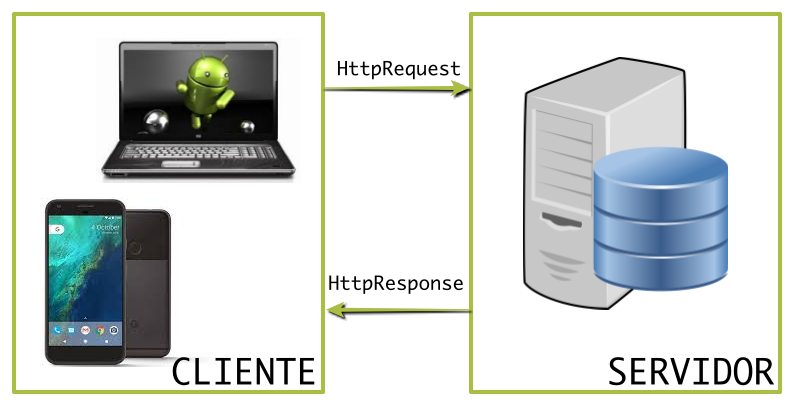
\includegraphics[width=0.70\linewidth, keepaspectratio]{img/arquitectura}
  \caption{Arquitectura Cliente-Servidor}
  \label{fig:arquitectura}
\end{figure}

% DISEÑO E IMPLEMENTACIÓN DEL SERVIDOR %
\section{Diseño e implementación del servidor} 
\label{sec:arquitecturaServidor}
Como hemos visto, la arquitectura del Servidor consta de dos grandes bloques: la lógica de Django y el almacenamiento de SQLite.  

\subsection{Lógica servidor: Django}
La lógica del proyecto My App Inventor está organizada en los siguientes directorios:
\begin{itemize}
	\item Projecto Django - \textbf{analyzeMyApp}: dentro nos encontraremos con los ficheros de configuración. En \textit{settings.py} indicaremos los parámetros principales del programa (directorios, idioma, base de datos \ldots), mientras que en \textit{wsgi.py} especificaremos las reglas de comunicación entre un servidor web y nuestra aplicación cuando despleguemos en producción. 
	\item Aplicación - \textbf{myAnalyzer}: en este directorio guardaremos la lógica de la aplicación, es decir, qué hacer cuando recibimos una petición, cómo será nuestro modelo de datos, qué pasos seguir al analizar un fichero recibido\ldots. En las siguientes secciones veremos más en detalle este apartado.
	\item Ficheros estáticos - \textbf{static}: donde están las imágenes, estilos CSS y pequeños JavaScript para utilizar con Bootstrap.  
	\item Plantillas - \textbf{templates}: incluye todas las plantillas HTML que formarán parte de la interacción del usuario con la aplicación. 
	\item Proyectos guardados - \textbf{saved\_projects}: además de guardar la información más relevante en base de datos, guardaremos una copia de seguridad de cada proyecto subido por el usuario en disco, así en caso de posibles ampliaciones de la lógica de evaluación, se podrá actualizar el resultado de forma transparente al usuario sin necesidad de que vuelva a cargar su programa de nuevo. 
\end{itemize}  
\begin{figure}[H]
  \dirtree{%
	.1 /.
	.2 manage.py.
	.2 analyzeMyApp.
	.3 \_\_init\_\_.py.
	.3 settings.py.
	.3 urls.py.
	.3 wsgi.py.
	.2 myAnalyzer.
	.3 \_\_init\_\_.py.
	.3 admin.py.
	.3 scoreMyAppMessages.py.
	.3 admin.py.
	.3 forms.py.
	.3 models.py.
	.3 urls.py.
	.3 apps.py.
	.3 scoreMyApp.py.
	.3 parser.py.
	.3 views.py.
	.3 errors.py.
	.3 tests.py.
	.2 static.
	.2 templates.
	.2 saved\_projects.
	}
  \caption{Directorio de archivos My App Inventor}
  \label{fig:dirarchivos}
\end{figure}

En líneas generales, el flujo de la aplicación sigue los pasos de la Figura~\ref{fig:flujoapp} y se define dentro del directorio \textbf{myAnalyzer}. Cuando un usuario registrado realiza una petición a la aplicación, se diferencia entre guardar un nuevo proyecto o cargar uno preexistente. Tras este paso, se procede al anáĺisis del programa y como paso final, se devuelve una respuesta con la clasificación obtenida. Durante todo el proceso, si se recibe una petición de un usuario no registrado, se redirige al mismo a la página de inicio. 
\begin{figure}[H]
  \centering
  \begin{tikzpicture}[node distance = 3cm]
	    % Place nodes
	    \node [block] (init) {Petición de usuario};
	    \node [decision, below of= init] (newproject) {¿Nuevo projecto?};
	    \node (AuxNode01) [text width=4cm, below of=newproject] {};
	    \node [block, right of=AuxNode01, node distance=3cm] (save) {Guardar en bbdd};
	    \node [block, left of=AuxNode01, node distance=3cm] (load) {Leer de bbdd};
	    \node [block, below of=AuxNode01] (analyze) {Analizar proyecto};
	    \node [block, below of=analyze] (end) {Enviar resultados};
	    % Draw edges
	    \path [line] (init) -- (newproject);
	    \path [line] (newproject) -| node [near start, above] {si} (save);
	    \path [line] (newproject) -| node [near start, above]{no}(load);
	    \path [line] (load) -- (analyze);
	    \path [line] (save) -- (analyze);
	    \path [line] (analyze) -- (end);
  \end{tikzpicture}
  \caption{Flujo principal My App Inventor}
  \label{fig:flujoapp}
\end{figure}
En el momento en que la aplicación recibe una petición HTTP del usuario con una URL concreta, ésta se mapea en el fichero \textit{urls.py}. Éste a su vez redirige la información a un procedimiento concreto de \textit{wsgi.py} en función de la operación a realizar: iniciar o cerrar sesión, actualizar datos de perfil, cargar un nuevo programa, ver los anteriormente guardados \ldots No todas las URLs son accesibles al usuario mediante la petición GET; por ejemplo, sólo podremos acceder a la vista que analiza los proyectos del usuario,\textit{views.showUserAnalyzeProjectsPage}, mediante una petición de tipo POST insertada en un formulario de la aplicación para mantener la integridad de los datos recibidos y controlar su contenido. Lo mismo ocurre con la vista \textit{views.showDownloadPage} en la que se accede a la petición POST a través de un formulario.
\begin{lstlisting}
urlpatterns = [
               url(r'^login/', views.showLoginPage),
               url(r'^logout/', views.showLogoutPage),
               url(r'^createprofile/', views.showCreateProfilePage),
               url(r'^userprofile/', views.showUserProfilePage),
               url(r'^download/', views.showDownloadPage),
               url(r'^updateprofile/', views.showUpdateProfilePage),
               url(r'^userprojects/', views.showUserProjectsPage),
               url(r'^analyze/', views.showUserAnalyzeProjectsPage),
               url(r'^$', views.showLoginPage),
               ]
\end{lstlisting}

Veamos en más detalle los diferentes procedimientos implicados en el proceso global que forman parte de la aplicación.
\subsubsection{Comunicación}
Como hemos comentado anteriormente, si un usuario no inicia sesión en la aplicación, se le devolverá siempre a la página inicial. Entre todas las librerías (o \textit{views}) que incorpora Django, utilizaremos el Sistema de Autenticación\footnote{\url{https://docs.djangoproject.com/en/1.11/topics/auth/default/}} para complementar las vistas que nos ayudarán a realizar las operaciones más comunes como iniciar o cerrar sesión (\textit{views.showLoginPage, views.showLogoutPage}), mantener la misma entre peticiones al servidor o comprobar si un usuario está conectado. 

Todas las peticiones se realizarán a través de los objetos HttpResponse\footnote{\url{https://docs.djangoproject.com/en/1.11/ref/request-response/}} de Django que manejan solicitudes GET y POST según corresponda. Por ejemplo, en la vista de inicio de sesión, se diferencia entre la solicitud de \textit{login} (GET), donde respondemos al usuario con un formulario en el que introducir sus datos de registro, y la recepción de los mismos en el método POST para autenticarle. 

Tras el inicio de sesión, el usuario será redirigido a la página principal donde podrá evaluar su código en función de si ya está subido a la aplicación o no, como vimos en la Figura~\ref{fig:flujoapp}. 

\begin{figure}[H]
  \centering
  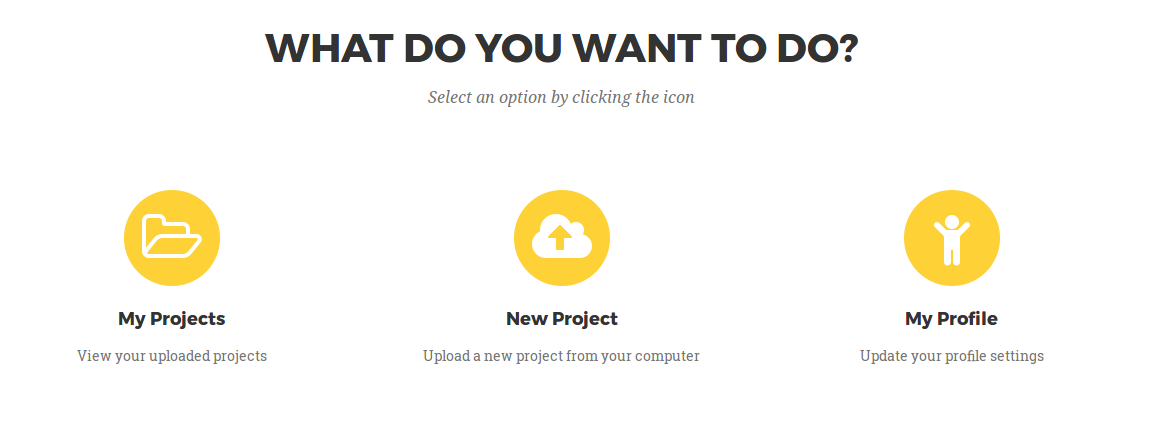
\includegraphics[width=\linewidth, keepaspectratio]{img/usercontent}
  \caption{Opciones disponibles}
  \label{fig:usercontent}
\end{figure}

Primero veamos el caso donde un programador quiere analizar su código por primera vez. La función \textit{views.showDownloadPage} devuelve en la primera petición (GET) un formulario en el que el usuario podrá buscar en su disco el fichero comprimido \textit{.aia} que previamente se ha descargado de su cuenta en App Inventor. Tras pulsar el botón Enviar, el navegador enviará una petición POST con el fichero al Servidor, donde se comprobará que no existe previamente para este usuario y descomprimirá, para posteriormente almacenar la información más relevante en base de datos. 

La estructura en la que App Inventor guarda la información sigue el esquema descrito en la figura~\ref{fig:dirappinventor}. En la carpeta \textit{assets} se almacenan los ficheros estáticos de la aplicación, como las imágenes y sonidos. En \textit{project.properties} se especifica la configuración del proyecto: versión del código, primera pantalla, tamaño\ldots. Y finalmente en el último nivel del directorio \textit{src} se encuentran la información relativa a los bloques utilizados (*.scm) y las lógicas que los relacionan (*.bky) por pantallas. Los datos más importantes para My App Inventor se encuentran en este último nivel y por ello serán los que guardemos en base de datos para su posterior análisis. 

\begin{figure}[H]
  \dirtree{%
	.1 /.
	.2 assets.
	.2 src.
	.3 appinventor.
	.4 settings.py.
	.5 ai\_loginappinventor.
	.6 nombrePrograma.
	.7 fichero.bky.
	.7 fichero.scm.
	.7 \ldots.
	.2 youngandroidproject.
	.3 project.properties.
	}
  \caption{Directorio App Inventor}
  \label{fig:dirappinventor}
\end{figure}

Si en un primer caso partíamos de un nuevo fichero de código, nuestra aplicación también permite al usuario guardar los proyectos guardados para poder volver a analizarlos en el futuro. Al llamar a la función \textit{views.showUserProjectsPage} el Servidor listará todos los programas almacenados para el usuario y éste podrá volver a obtener su clasificación. 

Tanto si partimos de un código nuevo como de uno ya existente, la última operación que hace My App Inventor es analizar el código. ¿Y por qué analizar algo que ya está puntuado? Pensando en futuras mejoras e implementaciones del algoritmo de análisis, de esta forma hacemos posible que el usuario siempre tenga su disposición la última versión del mismo con la clasificación más actualizada. Así no es necesario preprocesar todos los programas en base de datos en caso de actualización ya que ésta se realiza bajo demanda.

\subsubsection{Análisis de código}
El análisis de los programas del usuario se realiza a tres niveles: componentes, programación y usabilidad, cada uno con sus correspondientes subniveles. Como habíamos comentado en la sección anterior, en base de datos tendremos la información principal de las pantallas que forman cada proyecto. Para cada pantalla tenemos:

\begin{itemize}
  \item Fichero \textbf{.scm}: contiene los bloques añadidos al proyecto y sus propiedades en formato JSON (JavaScript Object Notation)\footnote{\url{http://www.json.org/}}, un formato de representación de objetos con una estructura sencilla basada en relaciones nombre-valor. En función del bloque utilizado tendremos unas propiedades u otras: posición (\textit{AlignHorizontal}), fondo (\textit{BackgroundColor}), tamaño (\textit{Width}) \ldots 
	\begin{figure}[H]
	  \centering
	  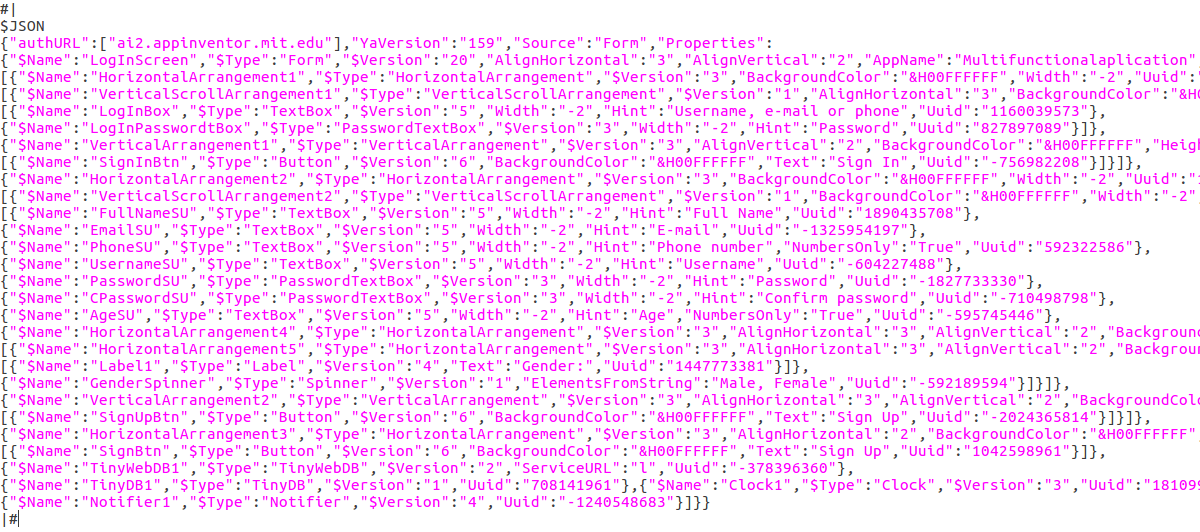
\includegraphics[width=\linewidth, keepaspectratio]{img/scmCode}
	  \caption{Ejemplo fichero .scm}
	  \label{fig:scmfile}
	\end{figure}
  \item Fichero \textbf{.bky}: en él se almacena en formato XML (Extensible Markup Language)\footnote{\url{https://www.w3.org/XML/}} todas las relaciones entre bloques activos y su funcionamiento. Será por tanto el principal fichero del que extraeremos la información estructural y funcional a analizar.
	\begin{figure}[H]
	  \centering
	  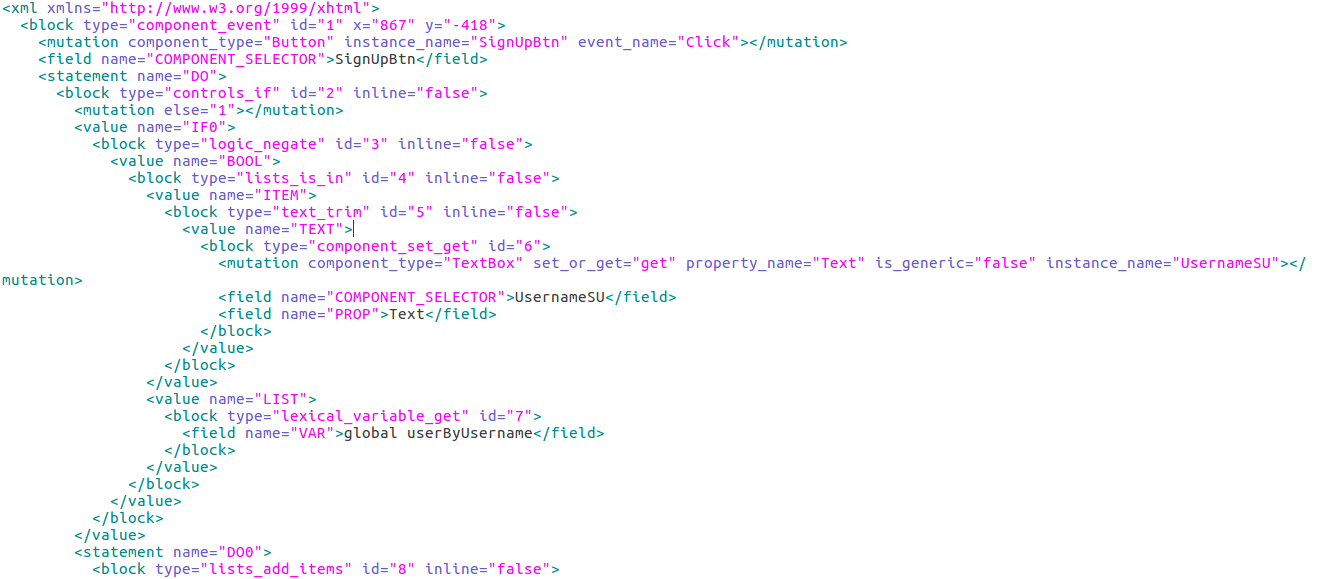
\includegraphics[width=\linewidth, keepaspectratio]{img/bkyCode}
	  \caption{Ejemplo fichero .bky}
	  \label{fig:bkyfile}
	\end{figure}
\end{itemize}

La función \textit{views.showUserAnalyzeProjectsPage} será la encargada de recibir la identificación del proyecto a analizar y responder al usuario con su evaluación. Tras consultar el contenido de las pantallas en base de datos, llamará a la función \textit{scoreMyApp.getScore} que analizará cada nivel individualmente. En este proceso, las funciones llamadas se han organizado en diferentes clases según su propósito:
\begin{itemize}
  \item \textbf{scoreMyApp}: contiene todas las funciones relativas a analizar el XML y obtener las estadísticas. Su función principal es \textit{scoreMyApp.getScore} y en esta sección nos centraremos en su análisis. 
  \item \textbf{scoreMyAppMessages}: procesa las clasificaciones y genera mensajes personalizados para el usuario.
\end{itemize}

Dentro de \textit{scoreMyApp.getScore} analizaremos cada nivel pantalla por pantalla, comparando los resultados en cada iteración de forma que la estructura final contenga toda la información del programa. 
\begin{lstlisting}
if componentLevels['Score'] > generalScore['ComponentLevels']['Score']:
# Update
generalScore['ComponentLevels']['Score'] = componentLevels['Score']

G1 = generalScore['ComponentLevels']['L1_components']
S1 = componentLevels['L1_components']
generalScore['ComponentLevels']['L1_components'] = returnUnion(G1,S1,0)
\end{lstlisting}
La clasificación se almacenará en un diccionario en el que guardaremos las estadísticas de cada nivel. Para obtener las puntuaciones individuales se obtiene una media con los niveles de las clasificaciones, mientras que la puntuación final es una media ponderada de los tres niveles a analizar. 
\begin{figure}
	\begin{center}
	    \begin{tabular}{| l | l | l | }
	    \hline
	    \textbf{Nivel} & \textbf{Subniveles} & \textbf{Ponderación} \\ \hline
	    ComponentLevels & Score,L1\_components,L2\_components,L3\_components & 45\% \\ \hline
	    ProgrammingLevels & Score,Flow,Data,Variable,Generalization & 45\% \\ \hline
	    ScreensLevels & Score,Screens & 10\% \\ \hline
            \end{tabular}
	\end{center}
	\caption{Estructura de la clasificación}
	\label{fig:scoreStructure}
\end{figure}
Los componentes utilizados y las habilidades de programación tienen un peso del 45\% cada uno en la media mientras que la usabilidad de la aplicación se lleva el 10\% restante al considerarse una característica a evaluar pero que no debe tener la misma importancia en la nota final pues es un concepto más de diseño que de habilidad en la programación.  

Para la evaluación de los \textbf{componentes} se han clasificado en tres niveles todos los bloques disponibles en App Inventor en función de su nivel de complejidad, independientemente de su naturaleza. Por ejemplo, en el nivel bajo nos encontramos con bloques tipo cuadro de texto y relojes, mientras que en el nivel alto tenemos componentes de Lego Mindstorms o bases de datos experimentales como FirebaseDB. 
\begin{figure}
	\begin{center}
	    \begin{tabular}{| l | p{0.85\linewidth} | }
	    \hline
	    \textbf{Subnivel} & \textbf{Bloques} \\ \hline
		Bajo & \textbf{InterfazUsuario} [Button CheckBox DatePicker Image Label ListPicker ListView Notifier Slider Spinner TextBox TimePicker] \textbf{Diseño} [HorizontalArrangement HorizontalScrollArrangement TableArrangement VerticalArrangement VerticalScrollArrangement] \textbf{Media} [ImagePicker] \textbf{Dibujo} [Ball Canvas ImageSprite] \textbf{Sensores} [Clock] \\ \hline
		Medio & \textbf{InterfazUsuario} [PasswordTextBox WebViewer] \textbf{Media} [Camcorder Camera Player Sound SoundRecorder SpeechRecognizer TextToSpeech VideoPlayer YandexTranslate] \textbf{Sensores} [AccelerometerSensor BarcodeScanner OrientationSensor Pedometer] \textbf{Social} [ContactPicker EmailPicker PhoneCall PhoneNumberPicker Sharing Texting Twitter] \textbf{Almacenamiento} [File TinyDB] \textbf{Conectividad} [ActivityStarter BluetoothClient]\\ \hline
		Alto & \textbf{Sensores} [GyroscopeSensor LocationSensor NearField ProximitySensor] \textbf{Almacenamiento} [FusionTablesControl TinyWebDB] \textbf{Conectividad} [BluethoothServer Web] \textbf{Lego} [NctDrive NctColorSensor NxtLightSensor NxtSoundSensor NxtTouchSensor NxtUltrasonicSensor NxtDirectCommands Ev3Motors Ev3ColorSensor Ev3GyroSensor Ev3TouchSensor Ev3UltrasonicSensor Ev3Sound Ev3UI Ev3Commands] \textbf{Experimental} [FirebaseDB]\\ \hline
            \end{tabular}
	\end{center}
	\caption{Componentes}
	\label{fig:componentsScore}
\end{figure}
Una vez definidos los tres niveles, con la función \textit{scoreMyApp.componentLevels\_Score} buscaremos todas las ocurrencias de cada tipo de bloque dentro de la pantalla, guardando los resultados en tres diccionarios:
\begin{lstlisting}
L1_found = {'UserInterface': UserInterface_L1_found,
                'Layout': Layout_L1_found,
                'Media': Media_L1_found,
                'Drawing': Drawing_L1_found,
                'Sensors': Sensors_L1_found}
    
L2_found = {'UserInterface': UserInterface_L2_found,
        'Media': Media_L2_found,
        'Sensors': Sensors_L2_found,
        'Social': Social_L2_found,
        'Storage': Storage_L2_found,
        'Connectivity':Connectivity_L2_found}
    
L3_found = {'Sensors': Sensors_L3_found,
        'Storage': Storage_L3_found,
        'Connectivity':Connectivity_L3_found,
        'Lego':Lego_L3_found,
        'Experimental':Experimental_L3_found}
\end{lstlisting}
Tras contabilizar el número de componentes total en cada subnivel, se asignará la puntuación de este módulo en función de la nota máxima alcanzada y guardaremos tanto la puntuación como el análisis para poder utilizarlos más adelante.   
\begin{lstlisting}
if c3 > 0 : # High score for complex components
score = 3
elif c2 > 0: # Medium score for complicated components
score = 2
else: # Low score for simple components
score = 1

results = {'Score':score,
       'L1_components':L1_found,
       'L2_components': L2_found,
       'L3_components': L3_found}
\end{lstlisting}

En la \textbf{programación} se revisarán competencias del usuario en distintas áreas de carácter abstracto como el control de flujo o el uso de funciones. Se han intentado agrupar a alto nivel las posibles etiquetas para poder organizarlas por funcionalidad y dentro de la misma, en los mínimos grupos, de manera que para cada subnivel tendremos siempre dos grupos globales que nos ayudarán a determinar la puntuación. 
\begin{figure}[H]
	\begin{center}
	    \begin{tabular}{| l | p{0.80\linewidth} | }
	    \hline
	    \textbf{Subnivel} & \textbf{Identificadores} \\ \hline
		Flow & component\_event controls\_ \\ \hline
		Data & lists component\_set\_get \\ \hline
		Variable & global\_declaration lexical\_variable\_get lexical\_variable\_set math\_ text\_ local\_declaration\_statement local\_declaration\_expression \\ \hline
		Generalization & procedures\_ is\_generic \\ \hline
            \end{tabular}
	\end{center}
	\caption{Programación}
	\label{fig:programmingScore}
\end{figure}
\begin{itemize}
  \item \textbf{Control de flujo} \textit{scoreMyApp.flow\_control}: identifica las expresiones lógicas para ejecutar ciclos, estructuras condicionales o eventos que dependen del comportamiento de otro componente o variable.
	\begin{itemize}
		\item Nivel alto: se incluyen expresiones lógicas y eventos dependientes. 
		\item Nivel medio: se incluyen expresiones lógicas o eventos dependientes.
		\item Nivel bajo: no incluye ningún control de flujo. 
	\end{itemize}
  \item \textbf{Gestión de datos} \textit{scoreMyApp.data\_control}: detecta el uso de listas para organización datos y asignación o modificación de valores a variables y componentes.
	\begin{itemize}
		\item Nivel alto: se incluyen listas y modificadores de variables. 
		\item Nivel medio: se incluyen listas o modificadores de variables.
		\item Nivel bajo: no se utilizan etiquetas de gestión de datos. 
	\end{itemize}
  \item \textbf{Representación de variables} \textit{scoreMyApp.variable\_control}: se tendrá en cuenta si el usuario utiliza declaraciones de variables tanto globales como locales y, en función del tipo de programa, expresiones matemáticas (sumas, potencias, operaciones de trigonometría\ldots) o expresiones relacionadas con textos (unión, convertir a mayúsculas, contiene\ldots).
	\begin{itemize}
		\item Nivel alto: se incluyen declaración de variables y funcionalidades de matemáticas o texto. 
		\item Nivel medio: se incluyen declaración de variables o funcionalidades de matemáticas o texto.
		\item Nivel bajo: no se utilizan métodos referenciados a variables. 
	\end{itemize}
  \item \textbf{Generalización} \textit{scoreMyApp.generalization\_control}: la optimización de código a través de funciones y la generalización de procesos para un mismo tipo de variable son características que todo buen programa debe tener ya que facilitan su lectura y permiten la reutilización procedimientos.   
	\begin{itemize}
		\item Nivel alto: se incluyen procedimientos y eventos genéricos para un mismo tipo de componente. 
		\item Nivel medio: se incluyen procedimientos (en esta ocasión se ha considerado que el uso de procedimientos es una funcionalidad básica e imprescindible)
		\item Nivel bajo: no se utiliza ningún tipo de mecanismo de generalización. 
	\end{itemize}
\end{itemize}
Al igual que en el nivel anterior, se guardarán todas las estadísticas e identificadores obtenidos en un diccionario además de la nota media de todas las subcategorías:
\begin{lstlisting}
results = {'Score':score,
       'Flow': flowCtrl,
       'Data': dataCtrl,
       'Variable': variableCtrl,
       'Generalization': generalizationCtrl}
\end{lstlisting}

Por último analizaremos la \textbf{usabilidad} extrapolándola al número de pantallas que forman la aplicación. Una de la características de las aplicaciones actuales es su simplicidad para el usuario. Incluir gran cantidad de pantallería y opciones reduce su usabilidad al convertirla en poco intuitiva. Si queremos mejorar la experiencia de usuario conviene que nuestro programa tenga un número suficientemente bajo de pantallas para que resulte fácil de utilizar pero no sea excesivamente sencillo para que no pierda funcionalidad. Tras estudiar las aplicaciones existentes en el mercado, en este apartado se han definido los siguientes niveles dentro de la función \textit{scoreMyApp.nScreens\_control}:

\begin{itemize}
	\item Nivel alto: entre 3 y 10 pantallas distintas. Ejemplos: Twitter, Facebook, Instagram\ldots
	\item Nivel medio: entre 1 y 3 pantallas. Ejemplos: Notas, Reloj, Calculadora
	\item Nivel bajo: una única pantalla o más de 10 pantallas. 
\end{itemize}

Tras el análisis de los componentes, técnicas de programación y usabilidad para todas las pantallas que componen el programa a analizar, obtendremos el siguiente esquema de resultados recopilando la máxima información posible, como se puede ver en la figura~\ref{fig:scoreAppInventor}.
\begin{figure}
  \dirtree{%
	.1 GeneralScore.
	.2 ComponentLevels.
	.3 Score.
	.3 L1\_components.
	.3 L2\_components.
	.3 L3\_components.
	.2 ProgrammingLevels.
	.3 Score.
	.3 Flow.
	.4 Component\_Events.
	.4 Control.
	.3 Data.
	.4 Lists.
	.4 ComponentSet.
	.3 Variable.
	.4 Variable.
	.4 Math.
	.4 Text.
	.3 Generalization.
	.4 Procs.
	.4 Generic.
	.2 ScreensLevels.	
	.3 Score.
	.3 Screens.
	}
  \caption{Resultados del análisis}
  \label{fig:scoreAppInventor}
\end{figure}
\subsubsection{Envío de resultados}
Volviendo a la vista encargada de obtener los resultados finales, \textit{views.showUserAnalyzeProjectsPage}, tras el análisis de los ficheros que componen el programa, llamaremos a las funciones de la clase \textit{scoreMyAppMessages}. En ella procesaremos toda la información y la mostraremos al usuario de forma intuitiva y simplificada a través de imágenes y mensajes de texto cortos. 
 
Gracias a la función \textit{scoreMyAppMessages.getScoreMsgs} obtendremos todos los datos necesarios que queremos mostrar al usuario a partir de los resultados vistos en el apartado anterior:
\begin{itemize}
	\item Nivel global - \textit{general\_score\_msg}: a partir de la puntuación general tendremos un mensaje que resumirá el nivel promedio de la aplicación. 
		\begin{lstlisting}
# General Score message
if score['Score'] == 3:
	general_score_msg = 'Great job! Your app has a HIGH score! Check out the different skills to improve it even more'
elif score['Score'] == 2:
	general_score_msg = 'Great job! Your app has a MEDIUM score! Check out the different skills to reach the next level'
else:
	general_score_msg = 'Ups! Your app has a LOW score. Check out the different skills to improve it'
		\end{lstlisting}
	\item Nivel por categoría - \textit{comp\_score\_msg, progr\_score\_msg, sched\_score\_msg}: componentes, programación y usabilidad mostrarán un mensaje personalizado en función de la puntuación media de sus subniveles. 
	\item Desglose de resultados por categoría - \textit{comp\_score\_info, progr\_score\_info, sched\_score\_info}: cada apartado incluirá la información más importante del mismo además de un consejo para mejorar el nivel actual. Dicho mensaje se mostrará siempre, pues aunque el usuario haya obtenido la máxima puntuación trataremos de motivarle para que incluya más complejidad a su programa o mayor diversidad de componentes. 
	\begin{itemize}
		\item Componentes: listará los bloques utilizados para conseguir este nivel.  
		\begin{figure}[H]
			  \centering
			  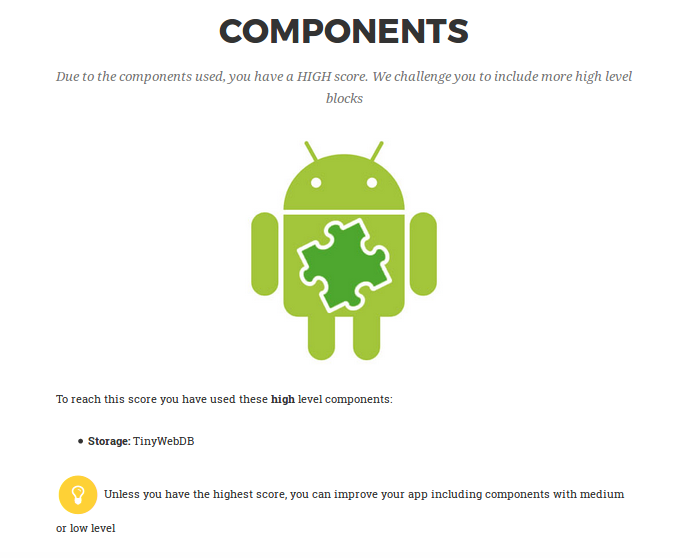
\includegraphics[width=0.50\linewidth, keepaspectratio]{img/componentsScore}
			  \caption{Resultados de la categoría Componentes}
			  \label{fig:compResults}
		\end{figure} 
		\item Programación: resumirá por categorías todos los identificadores añadidos al código junto con el número de veces que se utilizan de forma que el usuario pueda tener una visión global la estructura de su programa.      
		\begin{figure}[H]
			  \centering
			  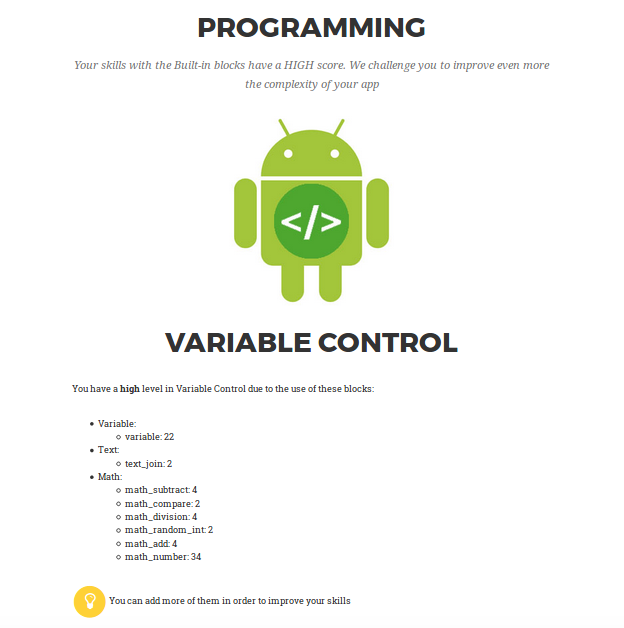
\includegraphics[width=0.60\linewidth, keepaspectratio]{img/programmingScore}
			  \caption{Resultados de la categoría Programación}
			  \label{fig:progrResults}
		\end{figure} 
		\item Usabilidad: muestra el número de pantallas que forman el programa.       
		\begin{figure}[H]
			  \centering
			  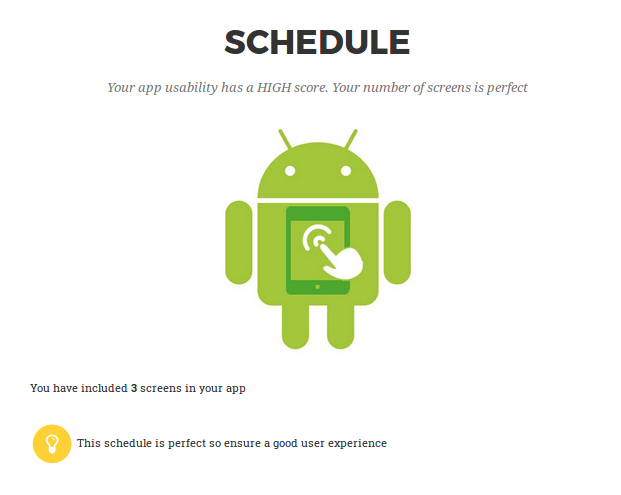
\includegraphics[width=0.50\linewidth, keepaspectratio]{img/schedScore}
			  \caption{Resultados de la categoría Usabilidad}
			  \label{fig:schedResults}
		\end{figure} 
	\end{itemize}
\end{itemize}

Una vez obtenidos todos los resultados, el siguiente pasó será enviarlos al navegador del usuario a través de la página \textit{analyzeAppCode.html}. En ésta se unen la mayoría de las tecnologías vistas en el capítulo Estado del Arte:
\begin{itemize}
	\item HTML: como estándar para definir la estructura básica del archivo, legible e interpretable por el navegador. Identificado en la siguiente etiqueta dentro del propio fichero:	
		\begin{lstlisting}[language=HTML]
<!DOCTYPE html>
		\end{lstlisting}
	\item CSS: antes de enviar el archivo HTML, parsearemos tanto los resultados del análisis como el estilo para integrarlos con el resto de valores de la página. Todos los formatos estarán definidos en diferentes ficheros .css almacenados estáticamente en el Servidor.  
		\begin{lstlisting}[language=HTML]


...

<link href="" rel="stylesheet">
		\end{lstlisting}
	\item JavaScript: gracias a este lenguaje de programación podemos implementar funciones dentro del HTML para que nuestra página sea más dinámica. Se utiliza por ejemplo, a la hora de ocultar o mostrar el menú:
	\begin{lstlisting}[language=HTML]
... 

// Highlight the top nav as scrolling occurs
$('body').scrollspy({
	target: '.navbar-fixed-top',
	offset: 51 });

// Closes the Responsive Menu on Menu Item Click
$('.navbar-collapse ul li a').click(function(){ 
    $('.navbar-toggle:visible').click(); });
	\end{lstlisting}
	\item Bootstrap: \textit{framework} que aúna el resto de tencnologías (HTML, CSS, JavaScript) y nos permite que la página se adapte a dispositivos móviles como se muestra en la figura~\ref{fig:dirappinventor}.
		\begin{lstlisting}
<!-- Bootstrap Core CSS -->
<link href="" rel="stylesheet">
		\end{lstlisting}
		\begin{figure}[H]
			  \centering
			  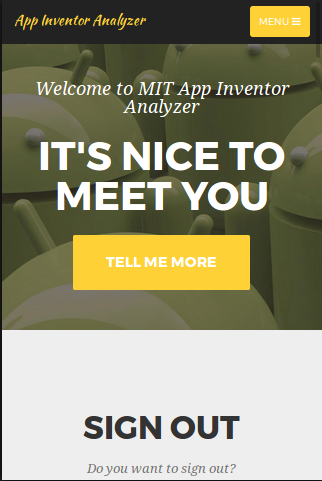
\includegraphics[width=0.30\linewidth, keepaspectratio]{img/mobileVersion}
			  \caption{Versión móvil con Bootstrap}
			  \label{fig:mobileVersion}
		\end{figure} 
		\begin{figure}[H]
			  \centering
			  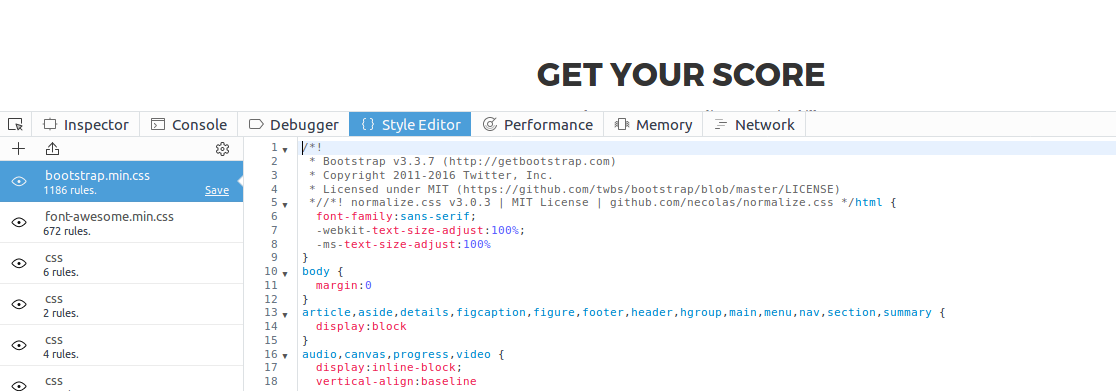
\includegraphics[width=\linewidth, keepaspectratio]{img/bootstrapDebug}
			  \caption{Petición de Bootstrap desde el navegador}
			  \label{fig:mobileVersion}
		\end{figure} 

\end{itemize}                                   

\subsection{Modelo de datos}
En la organización y uso de la información se han utilizado dos modelos en función de las características de los datos a guardar: 
\begin{itemize}
	\item Contenido no persistente: variables locales creadas durante la ejecución de los procesos en el servidor. 
	\item Contenido persistente: base de datos SQLite\footnote{\url{https://www.sqlite.org}} y almacenamiento en memoria.
\end{itemize}                                   

Como vimos en la sección anterior, los datos dinámicos donde se almacenan los resultados tras el análisis de código se guardan en una variable de tipo diccionario, donde se organizarán en pares clave-valor. En ella tendremos acceso tanto a las puntuaciones como a las prácticas de programación que las originan, ambas representadas en la figura~\ref{fig:scoreAppInventor}.

Por otro lado tendremos el almacenamiento en memoria estática de los programas subidos por cada usuario. Para ello se ha creado un sistema de directorios donde ir descargando el código y así poder tener acceso a él en el futuro en caso de actualizaciones del sistema de análisis. 

Los datos relativos a la información de usuario o los proyectos guardados por el mismo se guardarán en una base de datos, definida dentro de la aplicación en las clases de \textit{models.py}. Para todo lo relativo a la creación y autenticación de usuarios, Django dispone de objetos predefinidos\footnote{\url{https://docs.djangoproject.com/en/1.11/topics/auth}} que se han reutilizado añadiendo nuevas características. Para el caso del objeto User, que por defecto incluye como atributos primarios \textit{username, password, email, first\_name} y \textit{last\_name}, se ha usado de modelo base para la clase \textit{UserProfile} extendiéndolo de forma que también incluya el campo \textit{appinventorLogin}, necesario en la extracción de los ficheros comprimidos subidos por el usuario.
\begin{lstlisting}
class UserProfile(models.Model):
    user = models.OneToOneField(User)

    # The additional attributes we wish to include.
    appinventorLogin = models.CharField(max_length =254 )

    # Override the __unicode__() method to return out something meaningful!
    def __unicode__(self):
        return self.user.username    
\end{lstlisting}
Para almacenar los usuarios existentes en la aplicación, sus proyectos y el contenido de los mismos se han creado las siguientes clases: 
\begin{lstlisting}
class Users(models.Model):
    userID = models.IntegerField(primary_key=True) # user_id
    projects = models.ManyToManyField('Projects') # The user can load and analyze multiple projects

class Projects(models.Model):
    projectName = models.TextField(primary_key=True) # user.id_filename.name
    screens = models.ManyToManyField('Screens') # The project can include multiple screens
    projectProperties = models.TextField() # Project properties
    
class Screens(models.Model):
    scrID = models.TextField(primary_key=True) # user.id_filename.name_Screen number
    bky = models.TextField() # Blockly info
    scm = models.TextField() # Screen Description
\end{lstlisting} 
De esta forma un usuario puede tener varios proyectos que a su vez estarán compuestos por una o varias pantallas asociadas:
\begin{figure}[H]
  	\centering
	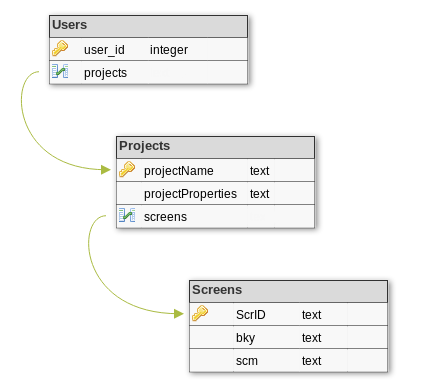
\includegraphics[width=0.80\linewidth, keepaspectratio]{img/databasediagram}
	\caption{Modelo de datos}
	\label{fig:databasemodel}
\end{figure}


% MANUAL DE USUARIO %
\section{Manual de Usuario} 
\label{sec:manualUsuario}
Al entrar en la aplicación la primera vista que se muestra al usuario es la de Bienvenida. El resto de opciones e información de la página se podrán visualizar a través de los links situados en el menú superior o desplazándose hacia abajo.
\begin{figure}[H]
  \centering
  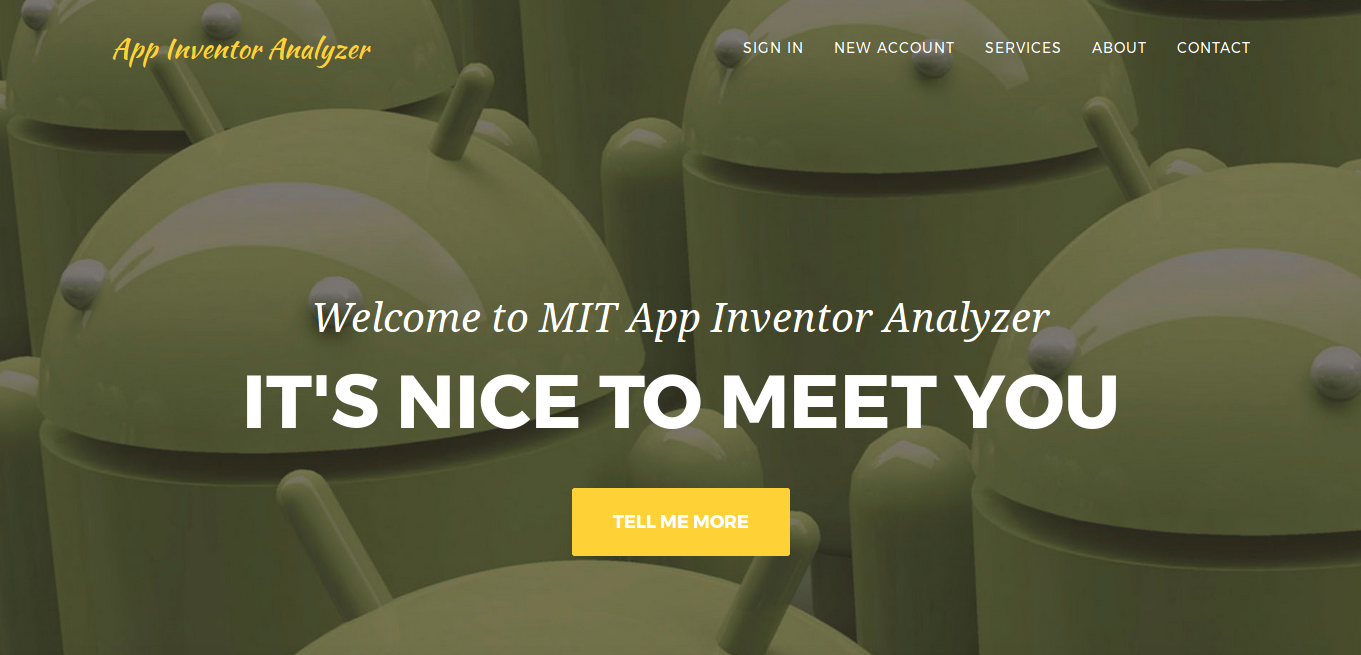
\includegraphics[width=\linewidth, keepaspectratio]{img/VistaPrincipal}
  \caption{Pantalla de Bienvenida}
  \label{fig:VistaPrincipal}
\end{figure}
En la pantalla de Inicio de Sesión el usuario podrá introducir su usuario y contraseña para poder acceder a su vista personal. 
\begin{figure}[H]
  \centering
  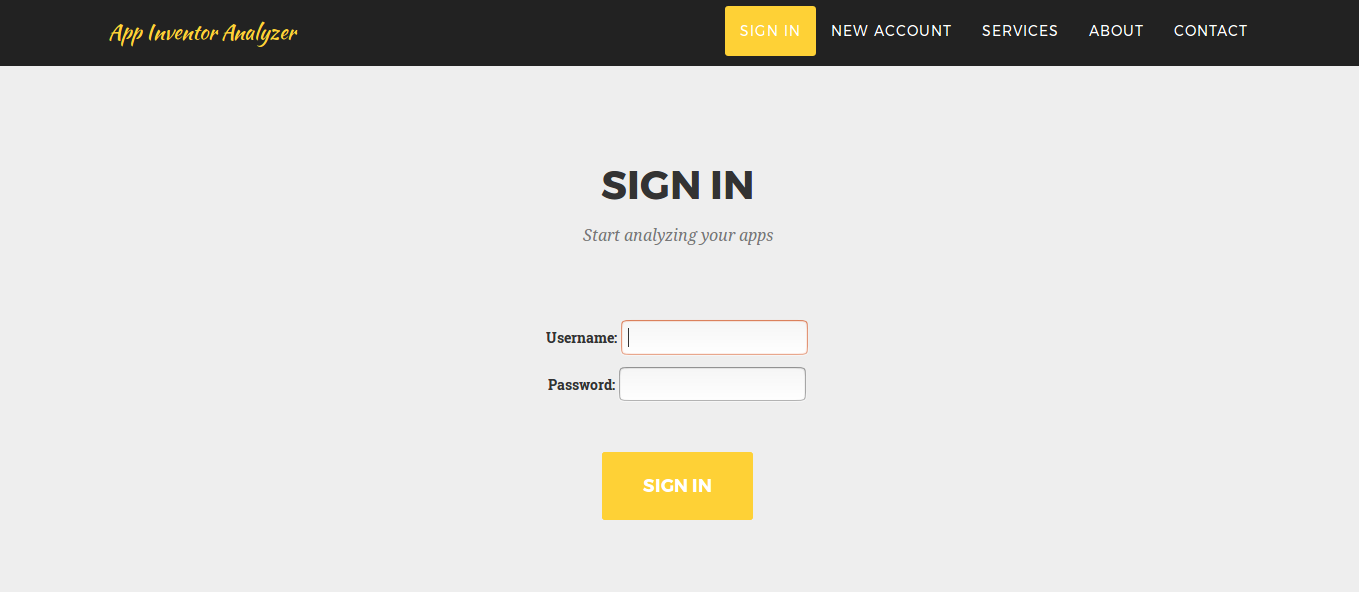
\includegraphics[width=\linewidth, keepaspectratio]{img/VistaPrincipal2}
  \caption{Pantalla de Inicio de Sesión}
  \label{fig:VistaPrincipal2}
\end{figure}
También se muestra información sobre los distintos aspectos que se estudian en la aplicación y un resumen de los pasos a seguir para analizar los proyectos:
\begin{figure}[H]
  \centering
  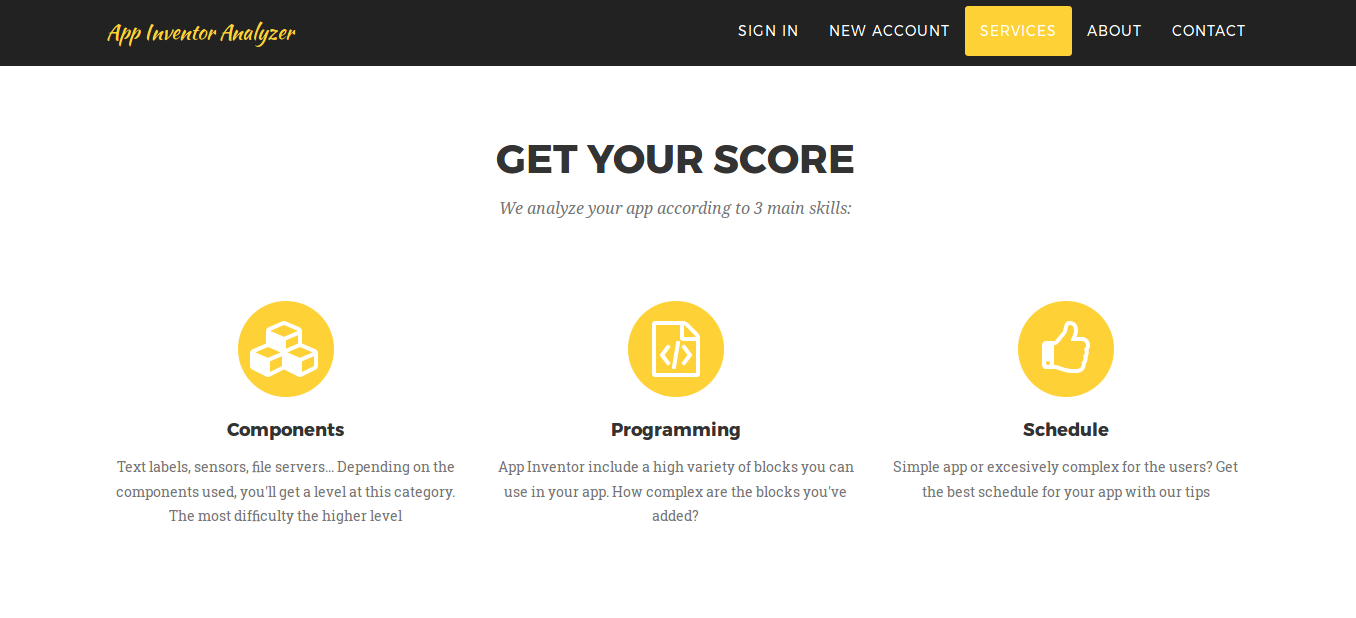
\includegraphics[width=\linewidth, keepaspectratio]{img/VistaPrincipal3}
  \caption{Pantalla Servicios}
  \label{fig:VistaPrincipal3}
\end{figure}
\begin{figure}[H]
  \centering
  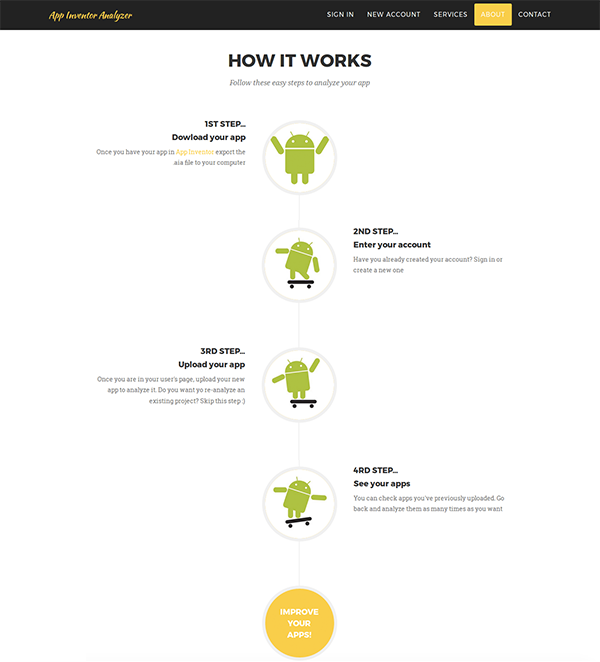
\includegraphics[width=0.60\linewidth, keepaspectratio]{img/About}
  \caption{Pantalla `Acerca de'}
  \label{fig:About}
\end{figure}

Si queremos utilizar My App Inventor y aún no nos hemos registrado, el primer paso será crear una cuenta de usuario. Para ello iremos a la opción `New Account' en el menú principal (Figura~\ref{fig:newAccountLink}), lo que abrirá una nueva pestaña en el navegador:
\begin{figure}[H]
  \centering
  
\includegraphics[width=0.40\linewidth, keepaspectratio]{img/newAccountLink}
  \caption{Link para crear una nueva cuenta}
  \label{fig:newAccountLink}
\end{figure}
Esta vista incluye todos los datos necesarios para crear una cuenta: nombre, email, contraseña\ldots. Será necesario especificar también el nick de usuario en App Inventor para poder leer correctamente los ficheros comprimidos.  
\begin{figure}[H]
  \centering
  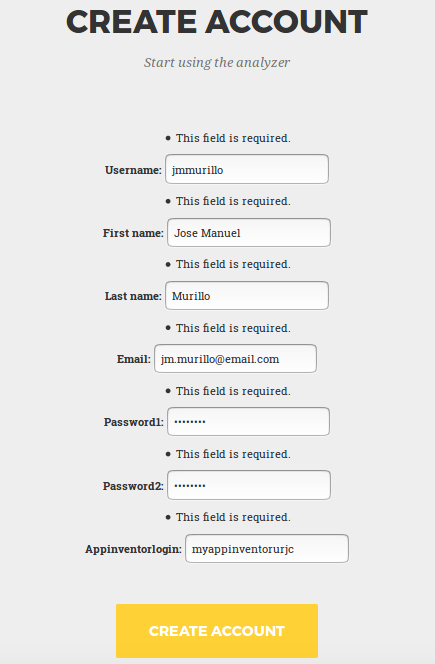
\includegraphics[width=0.55\linewidth, keepaspectratio]{img/createaccount}
  \caption{Creación de cuenta de usuario}
  \label{fig:createaccount}
\end{figure}
Si el usuario ya está registrado o las contraseñas no coinciden, la aplicación tiene implementadas una serie de validaciones que muestran un mensaje de error antes de crear la cuenta.
\begin{figure}[H]
  \centering
  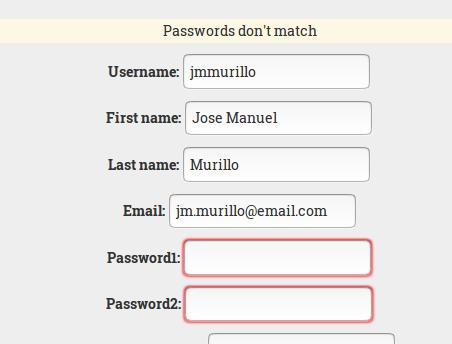
\includegraphics[width=0.60\linewidth, keepaspectratio]{img/invalidpassword}
  \caption{Mensaje de error por contraseña inválida}
  \label{fig:invalidpassword}
\end{figure}
También se informa si el registro ha finalizado correctamente:
\begin{figure}[H]
  \centering
  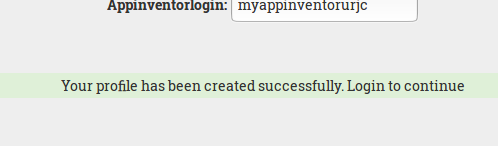
\includegraphics[width=0.70\linewidth, keepaspectratio]{img/createUserOK}
  \caption{Mensaje de confirmación al registrarse}
  \label{fig:createUserOK}
\end{figure}

Volviendo a la página principal, iniciaremos sesión en el apartado `Sign In', lo que redirigirá a la vista de la figura~\ref{fig:userView}. Nada más entrar nos muestra tres opciones: ver proyectos guardados, subir un nuevo proyecto o modificar los datos de nuestra cuenta. Tras seleccionar una de ellas la página ofrecerá el nuevo contenido (gracias a la tecnología AJAX podemos actualizar asíncronamente esta sección de la web).
\begin{figure}[H]
  \centering
  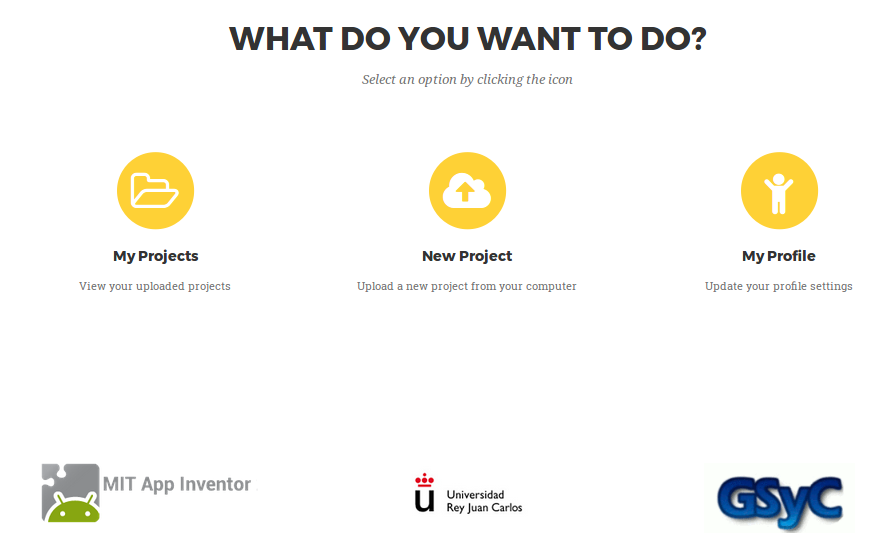
\includegraphics[width=0.90\linewidth, keepaspectratio]{img/userView}
  \caption{Opciones disponibles en vista de usuario}
  \label{fig:userView}
\end{figure}

Antes de comenzar a analizar un proyecto, veamos brevemente cómo actualizar nuestros datos de usuario. Seleccionando la opción `My Profile' tendremos acceso a la información susceptible de ser modificada. 
\begin{figure}[H]
  \centering
  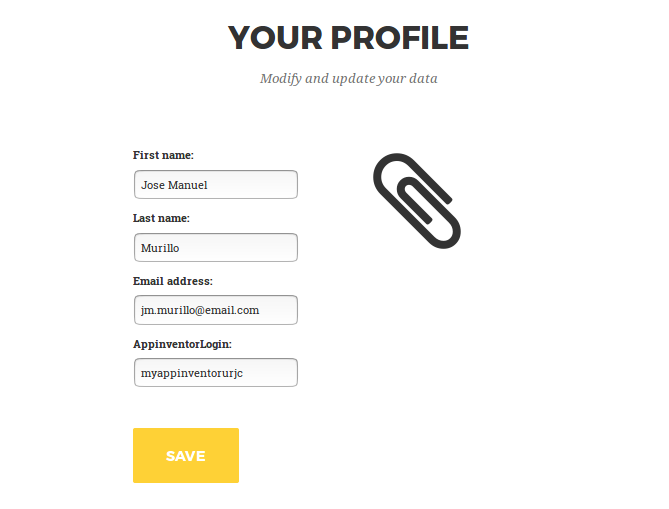
\includegraphics[width=0.70\linewidth, keepaspectratio]{img/profileUpdate}
  \caption{Actualización de datos de usuario}
  \label{fig:profileUpdate}
\end{figure}
Una vez realizado el cambio, nos aparecerá un mensaje de confirmación en la página principal.
\begin{figure}[H]
  \centering
  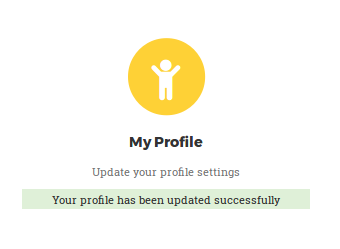
\includegraphics[width=0.60\linewidth, keepaspectratio]{img/profileUpdateOK}
  \caption{Mensaje de confirmación de actualización de datos de usuario}
  \label{fig:profileUpdateOK}
\end{figure}

Ahora que ya tenemos una cuenta, podemos subir nuestro primer proyecto. Para ello debemos ir a la opción `New Project' y buscaremos en nuestro disco el fichero \textit{.aia} previamente descargado de nuestra cuenta de App Inventor. Pulsamos `Load and Analyze` y ¡comienza el análisis!
\begin{figure}[H]
  \centering
  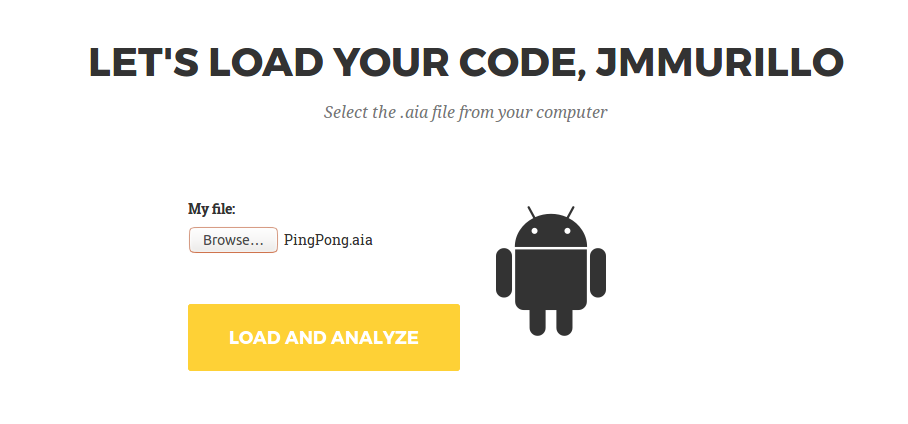
\includegraphics[width=\linewidth, keepaspectratio]{img/addNewProject}
  \caption{Añadir un nuevo proyecto}
  \label{fig:addNewProject}
\end{figure}
La aplicación nos redirigirá en segundos a una nueva vista, donde nos muestra la valoración general de los principales aspectos analizados. 
\begin{figure}[H]
  \centering
  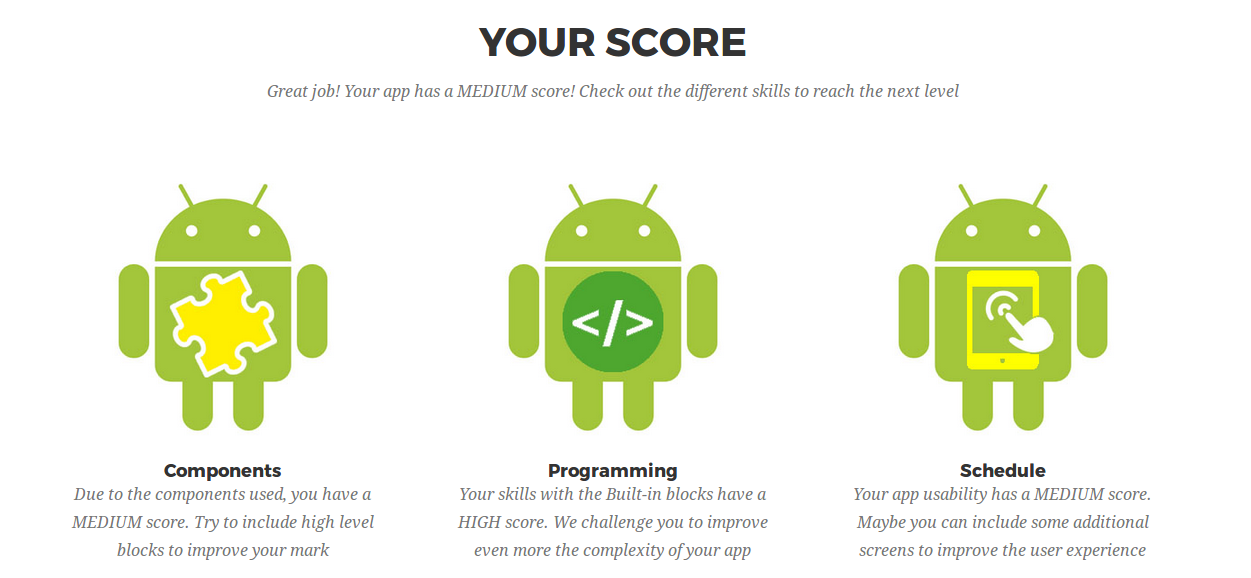
\includegraphics[width=\linewidth, keepaspectratio]{img/analysisResults}
  \caption{Resultados del análisis de nuestro proyecto}
  \label{fig:analysisResults}
\end{figure}
Si queremos ver el desglose de cada uno de ellos, simplemente haremos \textit{click} sobre cada opción para abrir una ventana emergente que mostrará la información desglosada como vimos en la figura~\ref{fig:componentsScore}.
\begin{figure}[H]
  \centering
  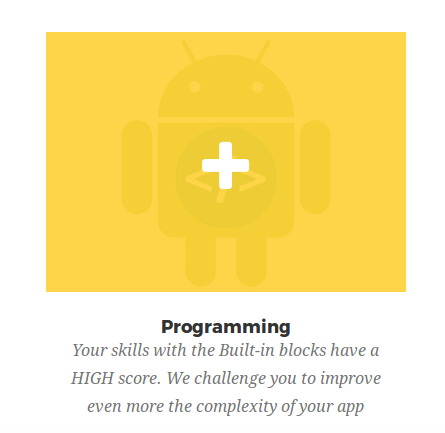
\includegraphics[width=0.60\linewidth, keepaspectratio]{img/popupoption}
  \caption{Ver desglose del análisis por categoría}
  \label{fig:popupoption}
\end{figure}

En caso de querer consultar el análisis de un proyecto que ya tenemos guardado con anterioridad, tendremos que ir a la opción `My Projects' del menú. En ella se listan todos los proyectos subidos por el usuario. Seleccionando uno de ellos y pulsando el botón `Lets Analyze' se mostrará de nuevo la información de la figura~\ref{fig:analysisResults}.
\begin{figure}[H]
  \centering
  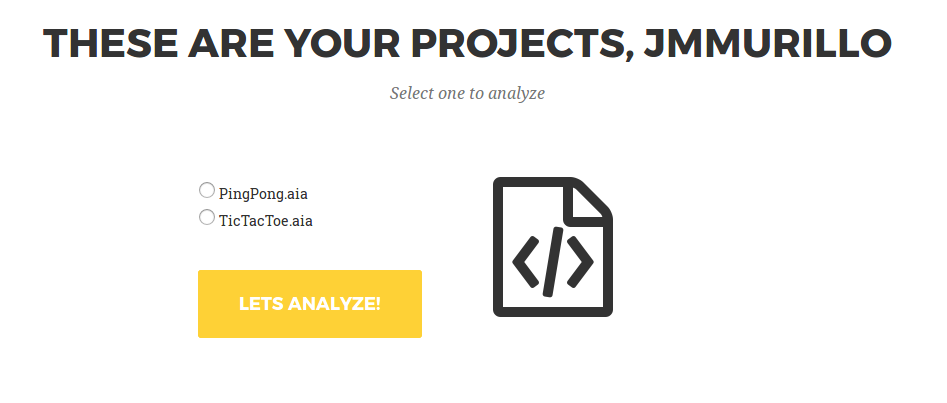
\includegraphics[width=\linewidth, keepaspectratio]{img/userproyects}
  \caption{Lista de proyectos guardados}
  \label{fig:popupoption}
\end{figure}

Para finalizar sesión y volver a la página general, basta con pulsar el botón `Sign out' situado en el menú superior y la aplicación nos redirigirá automáticamente a la vista principal como se muestra en la figura~\ref{fig:logoutOK}.
\begin{figure}[H]
  \centering
  
\includegraphics[width=0.50\linewidth, keepaspectratio]{img/logout}
  \caption{Botón para salir de sesión}
  \label{fig:logout}
\end{figure}
\begin{figure}[H]
  \centering
  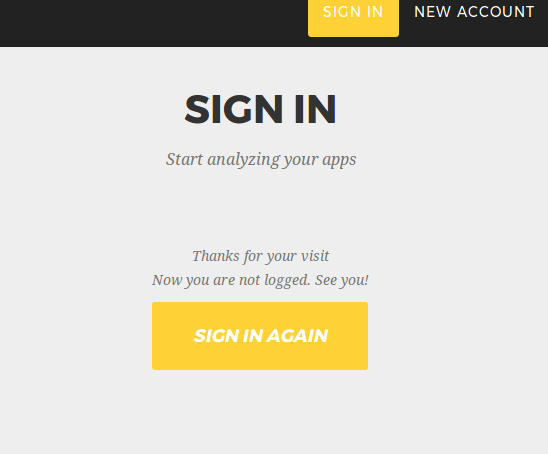
\includegraphics[width=0.70\linewidth, keepaspectratio]{img/logoutOK}
  \caption{Mensaje de confirmación de cierre de sesión}
  \label{fig:logoutOK}
\end{figure}


%%%%%%%%%%%%%%%%%%%%%%%%%%%%%%%%%%%%%%%%%%%%%%%%%%%%%%%%%%%%%%%%%%%%%%%%%%%%%%%%
%%%%%%%%%%%%%%%%%%%%%%%%%%%%%%%%%%%%%%%%%%%%%%%%%%%%%%%%%%%%%%%%%%%%%%%%%%%%%%%%
% RESULTADOS %
%%%%%%%%%%%%%%%%%%%%%%%%%%%%%%%%%%%%%%%%%%%%%%%%%%%%%%%%%%%%%%%%%%%%%%%%%%%%%%%%

\cleardoublepage
\chapter{Resultados}
A continuación vamos a analizar tres proyectos reales pertenecientes a la galería de App Inventor para ver la salida que obtenemos con el analizador.

\section{Nivel Alto:Multifunctional Aplication} 
\textit{Multifunctional Aplication} es un programa que incluye control de acceso, uso de eventos para modificar elementos en múltiples pantallas y uso de la base de datos TinyWebDB para guardar información. 
\begin{figure}[H]
  \centering
  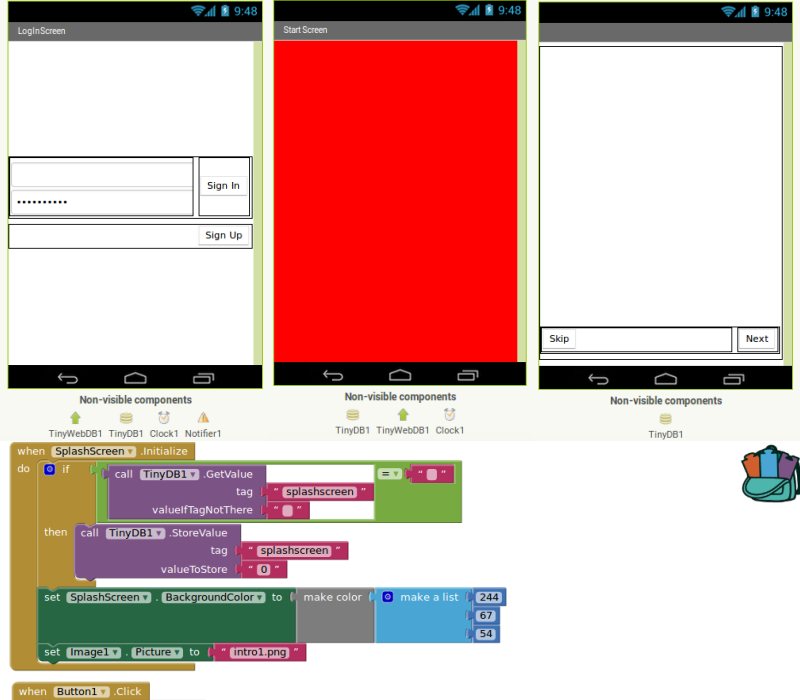
\includegraphics[width=0.60\linewidth, keepaspectratio]{img/MultiApp}
  \caption{Multifunctional Aplication: diseño}
  \label{fig:MultifunctionalApp}
\end{figure}
\begin{figure}[H]
  \centering
  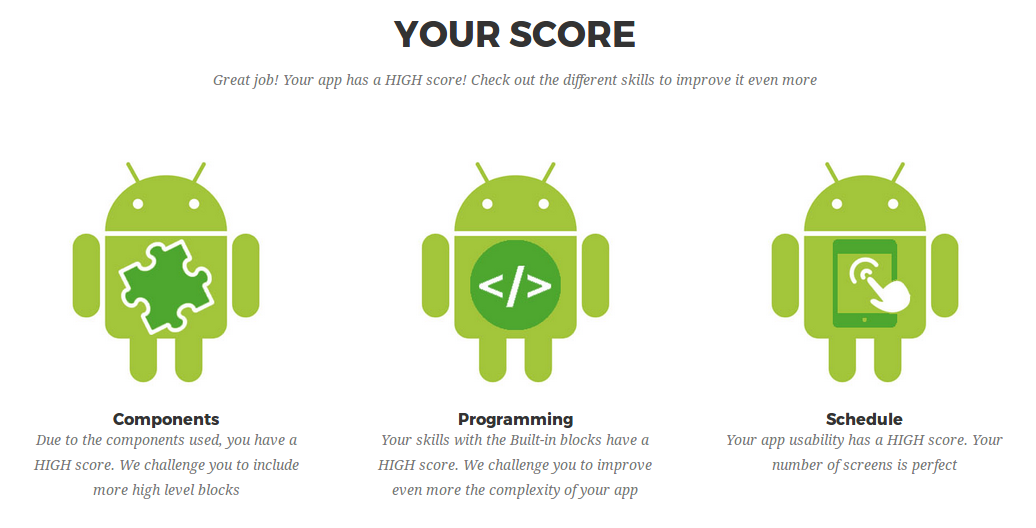
\includegraphics[width=\linewidth, keepaspectratio]{img/MultifunctionalAppGlobal}
  \caption{Multifunctional Aplication: clasificación general}
  \label{fig:MultifunctionalApp}
\end{figure}
Si analizamos el proyecto, My App Inventor le da una clasificación general Alta con el siguiente desglose de criterios:
\begin{itemize}
  \item Nivel Alto en Componentes: aunque incluye otro tipo de componentes, es el uso del almacenamiento con TinyWebDB el que le otorga cierta complejidad.
\begin{lstlisting}[language=]
To reach this score you have used these high level components:
    - Storage: TinyWebDB
Tip: Unless you have the highest score, you can improve your app including components with medium or low level
\end{lstlisting}
  \item Nivel Alto en Programación: control de variables, gestión de datos y control de flujo consiguen una clasificación alta, mientras que el uso de funciones y la ausencia de procedimientos generales hace que en generalización tenga un nivel medio. 
\begin{lstlisting}[language=]
VARIABLE CONTROL
You have a high level in Variable Control due to the use of these blocks:
    - Variable:
        - variable: 120
    - Text:
        - text_join: 8
        - text_trim: 20
        - text_isEmpty: 20
    - Math:
        - math_number: 16
Tip: You can add more of them in order to improve your skills

GENERALIZATION
You have a medium level in Generalization due to the use of these blocks:
    - Procedures:
        - procedures_callnoreturn: 8
        - procedures_defnoreturn: 4
    - Generalization: 0
Tip: Try to include both categories to improve your level

DATA MANAGEMENT
You have a high level in Data Management due to the use of these blocks:
    - Component Set:
        - component_set_get: 212
    - Lists:
        - lists_create_with: 20
        - lists_select_item: 16
        - lists_is_in: 16
        - lists_is_list: 8
        - lists_add_items: 8
Tip: You can add more of them in order to improve your skills
FLOW CONTROL 
You have a high level in Flow Control due to the use of these blocks:
    - Control:
        - controls_if: 44
    - Component_Events:
        - component_event: 28
Tip: You can add more of them in order to improve your skills
\end{lstlisting}
  \item Nivel Alto en Usabilidad: la inclusión de múltiples pantallas le otorga una puntuación alta. 
\begin{lstlisting}[language=]
You have included 3 screens in your app
Tip: This schedule is perfect so ensure a good user experience 
\end{lstlisting}
\end{itemize}

\section{Nivel Medio: Android Mash} 
\textit{Android Mash} es un juego sencillo que interactúa con el usuario a través de la pantalla táctil. Forma parte de los tutoriales incluidos en App Inventor para enseñar a incluir elementos básicos como una imagen de fondo, un sensor táctil, temporizador y comportamiento aleatorio. 
Como vemos en la figura~\ref{fig:AndroidMash}, está compuesto por una pantalla y pocos componentes que se relacionan a través de bloques condicionales y una función que genera números aleatorios. 
\begin{figure}[H]
  \centering
  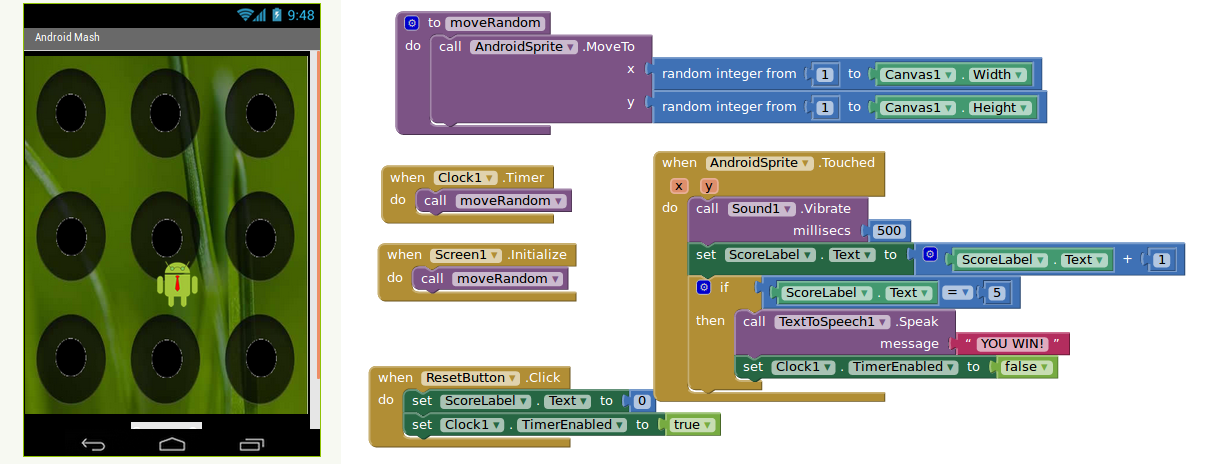
\includegraphics[width=\linewidth, keepaspectratio]{img/AndroidMash}
  \caption{Android Mash: diseño}
  \label{fig:AndroidMash}
\end{figure}
\begin{figure}[H]
  \centering
  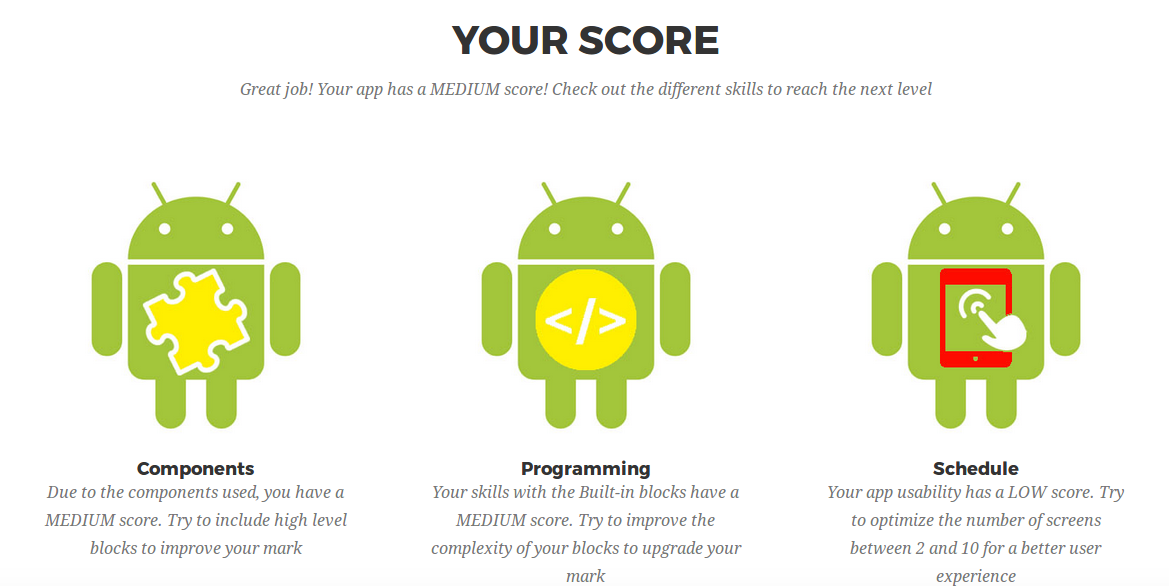
\includegraphics[width=\linewidth, keepaspectratio]{img/AndroidMashGlobal}
  \caption{Android Mash: clasificación general}
  \label{fig:AndroidMashGlobal}
\end{figure}
El análisis de este proyecto nos da un nivel medio general y los siguientes valores en el resto de criterios:
\begin{itemize}
  \item Nivel Medio en Componentes: aunque se trata de una interfaz sencilla, incluye elementos como sonidos y lectura de textos con voz lo que le dota de cierta complejidad a la aplicación.
\begin{lstlisting}[language=]
To reach this score you have used these medium level components:
    - Media: Sound,TextToSpeech
Tip: Try to include highest level blocks to improve your mark.
\end{lstlisting}
  \item Nivel Medio en Programación: en criterios como control de variables, generalización y gestión de datos tiene un nivel medio ya que incluye al menos uno de los identificadores de bloque necesarios. En control de flujo obtiene un nivel alto ya que utiliza tanto expresiones lógicas como dependencia de eventos. 
\begin{lstlisting}[language=]
VARIABLE CONTROL
You have a medium level in Variable Control due to the use of these blocks:
    - Variable:
	variable: 0
    - Text: 0
    - Math:
	math_random_int: 2
	math_add: 1
	math_compare: 1
	math_number: 6
Tip: Try to include more categories to improve your level

GENERALIZATION
You have a medium level in Generalization due to the use of these blocks:
    - Procedures:
        - procedures_callnoreturn: 2
        - procedures_defnoreturn: 1
    - Generalization:
        - generic: 0
Tip: Try to include both categories to improve your level

DATA MANAGEMENT
You have a medium level in Data management due to the use of these blocks:
    - Component Set:
        component_set_get: 8
    - Lists: 0
Tip: Try to include both categories to improve your level

FLOW CONTROL 
You have a high level in Flow Control due to the use of these blocks:
    - Control:
        controls_if: 1
    - Component_Events:
        component_event: 4
Tip: You can add more of them in order to improve your skills
\end{lstlisting}
  \item Nivel Bajo en Usabilidad: por el uso de una sola pantalla.
\begin{lstlisting}[language=]
You have included 1 screen in your app
Tip: With this schedule you have a simple app. Why not improve its design by adding one or two screens more? 
\end{lstlisting}
\end{itemize}

\section{Nivel Bajo: YOUB Analogic Clock} 
\textit{YOUB Analogic Clock} se trata de una aplicación sencilla donde se muestra un reloj analógico. Internamente está compuesto por componentes de tipo imagen que se relacionan a través de sencillos bloques de modificación de variables. 
\begin{figure}[H]
  \centering
  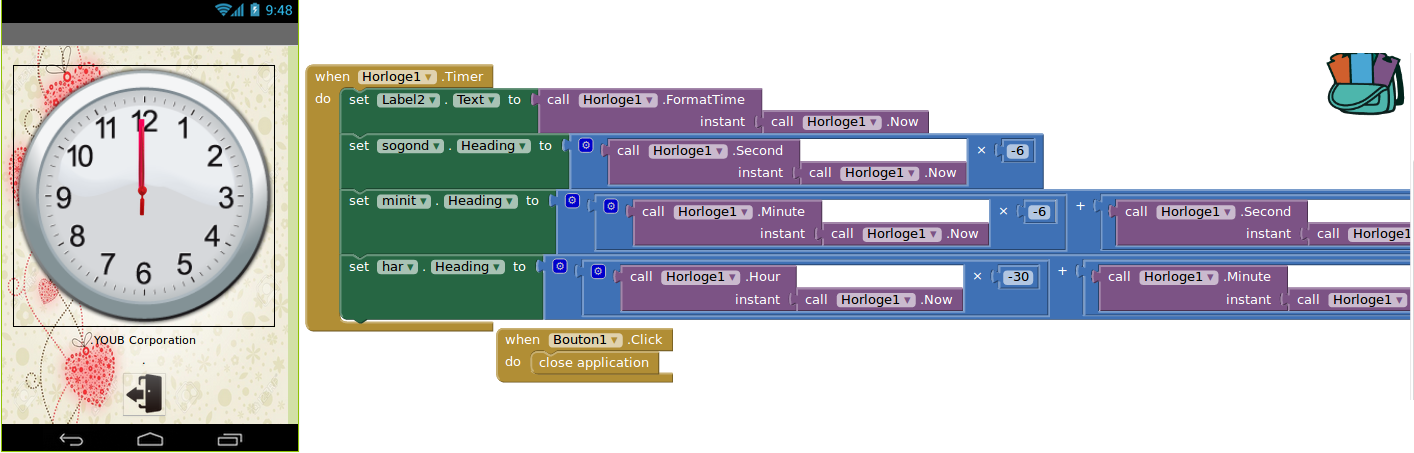
\includegraphics[width=\linewidth, keepaspectratio]{img/AnalogiClock}
  \caption{Analogic Clock: diseño}
  \label{fig:AnalogiClock}
\end{figure}
\begin{figure}[H]
  \centering
  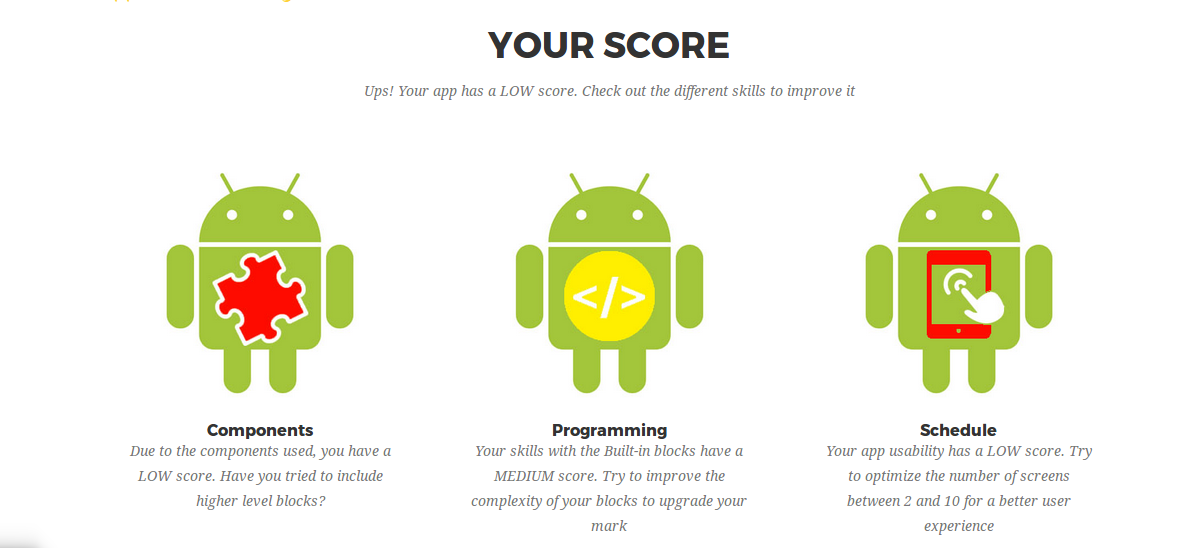
\includegraphics[width=\linewidth, keepaspectratio]{img/AnalogiClockGlobal}
  \caption{Analogic Clock: clasificación general}
  \label{fig:AnalogiClockGLobal}
\end{figure}
Tras analizar el proyecto, My App Inventor le da una clasificación general Baja con el siguiente desglose de criterios:
\begin{itemize}
  \item Nivel Bajo en Componentes: utiliza elementos sencillos como imágenes, un reloj y botones. 
\begin{lstlisting}[language=]
To reach this score you have used these low level components:
    - UserInterface: Button,Label
    - Drawing: ImageSprite
    - Sensors: Clock
Tip:Try to include high and medium level blocks to improve your mark.
\end{lstlisting}
  \item Nivel Medio en Programación: control de variables y gestión de datos tienen un nivel medio, generalización, un nivel bajo por la ausencia de procedimientos y control de flujo, alto por el uso de controles y eventos. 
\begin{lstlisting}[language=]
VARIABLE CONTROL 
You have a medium level in Variable Control due to the use of these blocks:
    - Variable:0
    - Text: 0
    - Math:
        - math_division: 2
        - math_add: 2
        - math_multiply: 3
        - math_number: 5
Tip:Try to include more categories to improve your level 

GENERALIZATION
You have a low level in Generalization due to the use of these blocks:
    - Procedures: 0
    - Generalization: 0
Tip:Try to include at least one of the categories to improve your level 

DATA MANAGEMENT
You have a medium level in Data management due to the use of these blocks:
    - Component Set:
        - component_set_get: 4
    - Lists: 0
Tip: Try to include both categories to improve your level

FLOW CONTROL
You have a high level in Flow Control due to the use of these blocks:
    - Control:
        - controls_closeApplication: 1
    - Component_Events:
        - component_event: 2
Tip: You can add more of them in order to improve your skills  
\end{lstlisting}
  \item Nivel Bajo en Usabilidad: sólo se incluye una pantalla. 
\begin{lstlisting}[language=]
You have included 1 screen in your app
Tip: With this schedule you have a simple app. Why not improve its design by adding one or two screens more? 
\end{lstlisting}
\end{itemize}

%%%%%%%%%%%%%%%%%%%%%%%%%%%%%%%%%%%%%%%%%%%%%%%%%%%%%%%%%%%%%%%%%%%%%%%%%%%%%%%%
%%%%%%%%%%%%%%%%%%%%%%%%%%%%%%%%%%%%%%%%%%%%%%%%%%%%%%%%%%%%%%%%%%%%%%%%%%%%%%%%
% CONCLUSIONES %
%%%%%%%%%%%%%%%%%%%%%%%%%%%%%%%%%%%%%%%%%%%%%%%%%%%%%%%%%%%%%%%%%%%%%%%%%%%%%%%%

\cleardoublepage
\chapter{Conclusiones}
\label{chap:conclusiones}
En este capítulo sea analizarán los objetivos planteados al inicio del proyecto, viendo cuáles se han cumplido y cuáles no. También haremos un repaso de los conocimientos adquiridos durante la carrera que me han sido de utilidad para realizar este proyecto  y qué he aprendido durante su creación. Por último, plantearemos las posibilidades de desarrollo de My App Inventor de cara a futuros proyectos. 

\section{Consecución de objetivos}
\label{sec:consecucion-objetivos}
El objetivo general del proyecto fue crear una plataforma donde poder evaluar los puntos fuertes y débiles de una aplicación creada en App Inventor. Este punto se ha cumplido con la creación de una web en la que el usuario, tras subir su código comprimido, puede ver el resultado del análisis y guardar su programa para futuras referencias. Además se han unido distintas tecnologías (Bootstrap, AJAX) para que la página sea más dinámica y siga las tendencias actuales. 

A continuación, veremos algunos obstáculos que fui encontrándome durante el desarrollo del proyecto y cómo los fui solventando:

\begin{itemize}
	\item La web de App Inventor requiere un registro para entrar y poder utilizar la aplicación. Dentro de la vista de usuario, tiene almacenados los proyectos guardados y en caso de querer descargar aplicaciones de otras personas, debemos antes duplicarlas en nuestro directorio. Al no existir una galería pública a la que acceder por una url simple, tuve que modificar el enfoque de Dr. Scratch y hacer que los usuarios sólo dispongan de la opción de subir un fichero comprimido desde su disco local. 
	\item Otro de los puntos que frenó el avance en la definición del algoritmo de análisis es el amplio abanico de opciones que podemos incluir en App Inventor y su escasa documentación. Al no encontrar una lista de posibilidades, opté por incluir todos los tipos de bloque en un programa y analizar el fichero resultante, estudiando distintas combinaciones y modificaciones. 
	\item Al no exisitir un \textit{plugin} como Hairball para el análisis del código de cada programa, al igual que en el punto anterior, desglosé los ficheros de código, creé un árbol con la información del XML y saqué patrones para posteriormente crear funciones como \textit{countBlocks} (contabiliza las etiquetas solicitadas), \textit{lookForBlocks} (busca bloques específicos) o \textit{listOfTypes} (crea una lista con los atributos buscados)
\end{itemize}

\section{Aplicación de lo aprendido}
\label{sec:aplicacion}
Si tuviera que destacar algún punto de la carrera de Telecomunicaciones sería la capacidad de razonar que me han aportado todas las asignaturas de programación. A parte de aprender a programar en distintos lenguajes, lo que te da una visión global, valoro el desarrollo de mi habilidad lógica y de razonamiento. Ambas han sido de gran ayuda en el ámbito laboral y por eso me gustaría poner mi granito de arena en dar a conocer iniciativas que fomentan aficiones positivas con alto valor añadido entre los jóvenes.  

Asignaturas como \textbf{Fundamentos de la Programación}, donde se asentaron las bases de todo lo que sé actualmente sobre programación y aprendí los conceptos básicos (condiciones, variables, bucles, funciones\ldots), o \textbf{Sistemas Telemáticos} en el que nos enseñaron la arquitectura Cliente-Servidor con sus comunicaciones, han sido importantes para llegar a comprender la estructura de un programa informático. Aunque si hay una asignatura clave que me haya empujado a realizar este proyecto ha sido \textbf{Servicios y Aplicaciones Telemáticas}, donde conocí el lenguaje de programación Python y obtuve los conocimientos necesarios para crear una página web más elaborada con tecnologías como CSS o AJAX. 

\section{Lecciones aprendidas}
\label{sec:lecciones_aprendidas}
Las lecciones aprendidas durante este proyecto han sido muchísimas, pero si tuviera que destacar alguna sería:
\begin{itemize}
  \item Hace unos meses aplicaciones como Scratch o App Inventor eran desconocidas para mí. Ahora que las conozco un poco más las recomiendo encarecidamente no sólo como plataformas para que los niños aprendan a programar, sino también los adultos, nunca es tarde para empezar nuevos retos.
  \item He podido profundizar y afianzar mis conocimientos sobre Python, Django y CSS.
  \item Al buscar la mejora de la presentación web, he aprendido a utilizar tecnologías como Bootstrap o AJAX.
  \item Dentro de la recopilación de información para incluir componentes a la página, he descubierto webs muy interesantes. Por ejemplo \textit{Font Awesome}\footnote{\url{http://fontawesome.io}}, un servidor gratuito de iconos en formato vector muy útil a la hora de decorar mensajes informativos en la página web ya que se formatean dentro del CSS. 
\end{itemize}

\section{Trabajos futuros}
\label{sec:trabajos_futuros}

My App Inventor abre una nueva línea de desarrollo para futuros proyectos. Algunas ideas para hacer crecer la aplicación serían:
\begin{itemize}
  \item Añadir un componente social en el que poder comparar mi puntuación con la de otros usuarios.
  \item Incluir gamificación con un sistema de recompensas si el usuario consigue ciertos logros en sus programas. 
  \item Creación de cuentas para profesores de cara a la utilización en clases de informática y como método de apoyo en la valoración
  \item Implementación de mecanismos de seguridad adicionales a los proporcionados por Django 
\end{itemize}

%%%%%%%%%%%%%%%%%%%%%%%%%%%%%%%%%%%%%%%%%%%%%%%%%%%%%%%%%%%%%%%%%%%%%%%%%%%%%%%%
%%%%%%%%%%%%%%%%%%%%%%%%%%%%%%%%%%%%%%%%%%%%%%%%%%%%%%%%%%%%%%%%%%%%%%%%%%%%%%%%
% APÉNDICE(S)

%\cleardoublepage
%\appendix
%\chapter{Manual de usuario}
%\label{app:manual}
%
%%%%%%%%%%%%%%%%%%%%%%%%%%%%%%%%%%%%%%%%%%%%%%%%%%%%%%%%%%%%%%%%%%%%%%%%%%%%%%%%

%%%%%%%%%%%%%%%%%%%%%%%%%%%%%%%%%%%%%%%%%%%%%%%%%%%%%%%%%%%%%%%%%%%%%%%%%%%%%%%%
%%%%%%%%%%%%%%%%%%%%%%%%%%%%%%%%%%%%%%%%%%%%%%%%%%%%%%%%%%%%%%%%%%%%%%%%%%%%%%%%
% BIBLIOGRAFIA %
%%%%%%%%%%%%%%%%%%%%%%%%%%%%%%%%%%%%%%%%%%%%%%%%%%%%%%%%%%%%%%%%%%%%%%%%%%%%%%%%

\cleardoublepage

% Las siguientes dos instrucciones es todo lo que necesitas
% para incluir las citas en la memoria
\bibliographystyle{abbrv}
\bibliography{memoria}  % memoria.bib es el nombre del fichero que contiene
% las referencias bibliográficas. Abre ese fichero y mira el formato que tiene,
% que se conoce como BibTeX. Hay muchos sitios que exportan referencias en
% formato BibTeX. Prueba a buscar en http://scholar.google.com por referencias
% y verás que lo puedes hacer de manera sencilla.
% Más información: 
% http://texblog.org/2014/04/22/using-google-scholar-to-download-bibtex-citations/

\end{document}L
